\documentclass[12pt]{iopart}
%Uncomment next line if AMS fonts required
%\usepackage{iopams}  
%\usepackage{natbib}
%\usepackage{amsmath, amssymb, amsfonts, amsthm, fouriernc, siunitx}
%\usepackage{amssymb, amsfonts, amsthm, fouriernc, siunitx}
\usepackage{amssymb, amsfonts,amsthm, fouriernc}
\usepackage{epsfig,graphics,graphicx}
\usepackage{color}

\newcommand{\eps}{{\varepsilon}}
\newcommand{\Pfus}{{P_{\textrm{\it\footnotesize fus}}}}
\newcommand{\hatPfus}{{\widehat{P}_{\textrm{\it\footnotesize fus}}}}

\newcommand{\bbf}{{\mathbf b}}
\newcommand{\ebf}{{\mathbf e}}
\newcommand{\jbf}{{\mathbf j}}
\newcommand{\kbf}{{\mathbf k}}
\newcommand{\ubf}{{\mathbf u}}
\newcommand{\vbf}{{\mathbf v}}
\newcommand{\xbf}{{\mathbf x}}
\newcommand{\Bbf}{{\mathbf B}}
\newcommand{\Ebf}{{\mathbf E}}
\newcommand{\Mbf}{{\mathbf M}}
\newcommand{\Sbf}{{\mathbf S}}
\newcommand{\Vbf}{{\mathbf V}}
\newcommand{\nablabf}{\mbox{\boldmath${\nabla}$}}
% !TeX spellcheck = en_US

% For highlighted modifications
%\newcommand{\newstuff}[1]{\color{red}{#1}\color{black}}
\newcommand{\newstuff}[1]{\color{blue}{#1}\color{black}}


\begin{document}

\title{Impact of scaling laws on tokamak \newstuff{reactor } dimensioning}

\author{Y. Sarazin, J. Hillairet, J.-L. Duchateau, K. Gaudimont, R. Varennes, X. Garbet, Ph. Ghendrih, R. Guirlet, B. P\'egouri\'e, A. Torre}

\address{CEA, IRFM, Saint-Paul-lez-Durance, F-13108, France.}
\ead{yanick.sarazin@cea.fr}
\vspace{10pt}
\begin{indented}
\item[\today]
\end{indented}

\begin{abstract}
A simple and comprehensive method is derived and used to quantify the impact of scaling laws on tokamak dimensioning. Assuming prescribed geometrical coefficients, we find the ensemble of possible triplets $R$, $B$ and normalized beta $\beta_N$ which allow one to reach target fusion gain $Q$ and fusion power $\Pfus$, at arbitrary Greenwald fraction. The model is generic and derived for any scaling law of the energy confinement time. Using the IPB98(y,2) scaling law [ITER Physics Expert Group on Confinement and Transport and Confinement Modeling and Database and ITER Physics Basis Editors, \emph{Nucl. Fusion} 39 (1999) 2175] leads to ITER specifications, as expected. The recently proposed new scaling law for H-mode plasmas (DS03, [A.C.C. Sips et al., \emph{Nucl. Fusion} 58 (2018) 126010]) is shown to lead to modest changes to the dimensioning, except for $B$ which could be significantly smaller for the same target performance. The impact on the dimensioning of critical exponents of the scaling law -- both regarding engineer and dimensionless variables -- is assessed, pushing for their determination with refined accuracy. Finally, the method is applied to a DEMO-like machine. The DS03 scaling law is found to have favorable consequences on the dimensioning as compared to IPB98(y,2), provided one is able to operate at larger $\beta_N$. Importantly, the opposite scaling of both scaling laws with respect to the aspect ratio are shown to have tremendous consequences on the optimal choice of this critical parameter. 
\end{abstract}

%
% Uncomment for keywords
%\vspace{2pc}
%\noindent{\it Keywords}: XXXXXX, YYYYYYYY, ZZZZZZZZZ
%
% Uncomment for Submitted to journal title message
\submitto{\NF}
% 
% For two-column output uncomment the next line and choose [10pt] rather than [12pt] in the \documentclass declaration
%\ioptwocol
%

%===================================================================
\section{Introduction}
%===================================================================
The aim of fusion energy research is to provide fusion power  $\Pfus$ minimizing the required auxiliary heating power, $P_{aux}$, and therefore maximizing the amplification factor $Q = \Pfus/P_{aux}$. Designing next step experiments in ITER or a tokamak reactor combines technological and physics based constraints. Given a target fusion power $\Pfus$ what are the constraints that determine the key parameters, namely the size and magnetic field of a tokamak reactor? The answer is not straightforward, and optimum trade-off must be addressed. Technological issues are surely among the important ones, either regarding thermal and neutron loads on divertor and plasma wall materials, respectively \cite{Federici2017, Siccinio2018}, or the maximum magnetic field which can be delivered by industrial-type super-conductors \cite{Duchateau2014}. In that respect, an effort is devoted to explore the impact on the design of DEMO -- the possible successor of ITER on the route towards a fusion power plant \cite{Federici2017} -- of uncertainties regarding both critical engineering parameters \cite{Coleman2016,Reux2018} and that of the tritium cycle \cite{Coleman2019}.
Regarding plasma physics issues, the route to fusion energy using magnetic confinement is paved with experimental findings, in particular via scaling laws. Uncertainties are significant \cite{Zohm2013}, especially when compared to that introduced by technology. At the crux of the design effort, the fusion gain $Q$ is inherently governed by the energy confinement time. The knowledge of the latter is based on an empirical scaling law.  Extrapolation from present experimental data must be done to address the operating point of ITER and even more of DEMO. The best scaling laws exhibit standard deviations of about $16\%$. Although this overall reliability might look acceptable at first sight, it actually masks much larger uncertainties with respect to some critical parameters for which a sufficiently unbiased data base is still lacking. \\

The objective of this paper is to investigate how the form of the scaling law of the energy confinement time $\tau_E$, dependencies and uncertainties, impacts the design of a tokamak aiming at burning plasma operation, typically $Q \ge 5$. The approach is based on a 0-dimensional analysis (with some refinement to account for temperature peaking) allowing for a step-by-step derivation of all constitutive relations, including the comprehensive computation of all the constants required in determining quantitative parameters. The \newstuff{calculation } is generic with formal expressions, hence allowing further investigation, e.g. by considering different scaling laws or machine specifications. Particular attention is payed to size and magnetic field because these drive the cost and in many respects feasibility of a given design. Two main aspects are considered for a given a reference empirical scaling laws for the energy confinement time proposed in the literature: on the one hand how prescribed target fusion performance translate in terms of machine size, and on the other hand how the uncertainties associated to the scaling laws propagate into a range of machine sizes. In that respect, a known feature of the energy confinement time scaling law is the strong dependence in the dimensionless parameter $\rho_*$, ratio of the characteristic Larmor gyration length to the tokamak minor radius. Results obtained here indicate that even a small uncertainty on this dependence has a big impact on the required size. Calculation of this parameter dependence and related uncertainty can then be traced in the empirical data. One can then define specific investigation steps to reduce the uncertainty with dedicated experiments and simulations \cite{Caschera2019}. The present paper aims at giving pedagogical insight into the art of tokamak design as well as providing a tool to investigate some aspects of uncertainty propagation. It proves effective in recovering main findings and unraveling new features. \\

The empirical scaling law is characterized by a dependence on a large set of variables. Some are dimensionless, typically those describing the geometry of the magnetic surfaces. The others can be split into engineering parameters, those that are directly set by the machine operation, while others are physical parameters that result from plasma performance. The two sets are combined to define a set of dimensionless parameters, $\rho_*$, $\nu_*$ and $\beta$, the latter two being the collision frequency normalized to the transit time frequency and the ratio of the kinetic pressure over the magnetic pressure, respectively. Setting the geometry and assuming the fusion cross section to exhibit a quadratic dependence on the thermal energy, it is possible to restrict the unknowns to four parameters, conveniently the plasma density and thermal energy and two critical engineering parameters, namely the torus major radius and magnetic field. The procedure that is followed is to set the output fusion power, and, via a target fusion gain to prescribe the energy confinement time. This yields two constrains. The physical parameters density and temperature are then changed into two parameters that are used to evaluate the distance to known operating limits, density limit on the one hand and MHD limit on the other hand. Due to the quadratic dependence of fusion power on the density, one can consider that a natural constraint is to set the density close to the limit, typically 20 \% below the limit. The output of the calculation is then sets of values of major radius and magnetic field determined in terms of the parameter describing the MHD limit. This well defined process provides a generic framework for such studies.  \\

The paper is organized as follows. The constitutive relations are recalled in section \ref{sec:Key Physics input for reactor design}, where the explicit expressions of all the constants are derived. Section \ref{sec:Tokamak_dimensioning} shows how these relations govern the dimensioning of tokamak, mainly in terms of magnetic field $B$ and major radius $R$. In particular, the ITER characteristics are recovered provided the IPB98(y,2) scaling law for $\tau_E$ is considered \cite{ITERphysics_chap2}. The impact on the dimensioning of the newly proposed scaling law for ELMy H-mode plasmas is also addressed \cite{Sips2018}, as well as that of the scaling exponents of the critical dimensionless variables $\rho_*$, $\nu_*$ and $\beta$. Finally, implications on the characteristics of DEMO are briefly discussed, including a critical discussion regarding the dependence on the aspect ratio.

%===================================================================
\section{Key Physics input for reactor design} 
\label{sec:Key Physics input for reactor design}
%===================================================================
\emph{Preliminary remark regarding the choice of units:} In the following, unless specified, the International System of Units (SI) is used. However, for simplicity, some of the most used parameters are \emph{not} expressed in SI units, these are identified with hats ``$\widehat{...}$''. The following specific units are employed:
% 
\begin{itemize}
	\item $\widehat n$ is the density in $10^{19}\, {m^{-3}}$: 
	$\widehat n = 10^{-19}\,n_{{[m^{-3}]}}$
	\item $\widehat T$ and $\widehat E$ are the thermal energy and any other energy, respectively, expressed in $keV$: $\widehat T = (10^{-3}k_B/e)\, T_{[K]}$ and $\widehat E = (10^{-3}/e)\, E_{[J]}$\\(with $k_B$ the Boltzmann's constant and $e$ the elementary electric charge)
	\item $\widehat I_p$ is the plasma current in MA: $\widehat I_p = 10^{-6}\, I_{p\,[A]}$
	\item $\widehat P$ is the power in MW: $\widehat P = 10^{-6}\, P_{[W]}$
\end{itemize}
%
\newstuff{In addition, $M$ is the mass in Atomic Mass Unit. } Also, for the sake of simplicity and in marked difference with respect to advanced system codes \cite{Kovari2014,Reux2015}, flat profiles of density and current are considered. However, taking into account the temperature peaking has proven to be important to recover the target performance of ITER working conditions.

Among the available control parameters, some are chosen as input parameters while others will be the output of the analysis. For the sake of simplicity, the geometry of the magnetic surfaces is given. Consequently, several dimensionless control parameters specifying the shape, aspect ratio -- $A\doteq R/a \doteq \eps^{-1}$, elongation $\kappa$ and triangularity $\delta$ -- are chosen to be input parameters. The target fusion performance of the machine is also chosen to be prescribed since it is a primary objective of a fusion reactor. We therefore set as inputs the fusion power $\Pfus$ and fusion gain $Q$ -- equivalently the auxiliary heating power. \\

In steady state conditions and for chosen nuclear fusion reaction, here D-T fusion, the gain $Q$ and $\Pfus$ determine the energy confinement time $\tau_E$. The latter is assumed to follow a known scaling law, which depends on density, temperature, magnetic field and major radius, while the fusion power depends on density and temperature. Two relationships are thus obtained that constrain the set of parameters. The following steps of the analysis are standard, thus to a large extent comparable to that followed by H. Zohm and coworkers \cite{Zohm2017} (a major difference being that we explicitly derive and give the expressions of all the constants). 
Among the four independent control parameters, the magnetic field and major radius are engineering parameters that can readily be addressed in terms of feasibility issues. Indeed, technological limits -- limits regarding industrial superconductors, mechanical resistance to stresses and forces, limits regarding the acceptable power heat flux impacting plasma facing components \cite{Siccinio2018} -- and economical considerations -- the cost of the machine is basically expected to scale like the magnetic energy, i.e. $B^2 R^3$ -- set clear bounds to what can reasonably be achieved. Conversely, density and temperature are constrained by plasma physics issues. In fact, one connects here these two parameters to critical parameters that appear to bound the operational space of present experiments. The two main soft limitations that we consider are the Greenwald density limit and the so-called normalized beta ($\beta_N$) limit. As a matter of fact, these allow one to define upper bounds -- although soft ones -- to the accessible density and temperature. In the following we show how the set of engineering parameters can be reduced to the four independent parameters and we then relate these to the two chosen operational limits. We also bridge these parameters to the dimensionless parameters.


%-------------------------------------------------------------------
\subsection{Density and Greenwald limit} \label{subsec:density_Greenwald}

As stated in a topical review on the subject \cite{Greenwald2002}, \emph{``%in addition to the operational limits imposed by MHD stability on plasma current and pressure, 
an independent limit on plasma density is observed in confined toroidal plasmas. [...] In tokamaks, [...] there is strong evidence linking the limit to physics near the plasma boundary [...]''}. As a matter of fact, the so-called Greenwald density $n_G$ is not a sharp density limit, rather a soft one, since discharges with peaked density profiles can well operate above this value. So far, there is no widely accepted, first principles model for the density limit. Yet, the focus is currently either on mechanisms which lead to strong edge cooling, or on collisionality enhanced turbulent transport.

From \cite[eq.(14.146)]{Freidberg2007}, the most common empirical scaling for (line-averaged) density limit is the following:
\begin{equation}
\widehat n_G \doteq C_n \frac{\widehat I_p}{\varepsilon^2 R^2}
\label{eq:greenwald_density}
\end{equation}
with $R$ the major radius of the tokamak, $\widehat I_p$ the plasma current and $C_n = 10/\pi \approx 3.18$.
Integrating the Maxwell-Amp\`ere equation over the whole plasma poloidal cross-section and using Stokes' theorem provides the relationship between $I_p$ and the magnetic field ($\mu_0 = 4\pi\, 10^{-7} {H.m^{-1}}$):
\begin{equation*}
\int_\mathcal{S} (\nablabf\times \Bbf) \cdot \mathbf{dS}
= \mu_0 \int_\mathcal{S} \jbf \cdot \mathbf{dS}
\to
\oint_\mathcal{C} \mathbf{B} \cdot \mathbf{d\ell} = \mu_0 I_p
\end{equation*}
Let us denote $L_{cs}=2\pi a \times F$ the length of the poloidal cross-section, with $F$ some factor depending on the plasma shape. $F=1$ for circular plasmas. If accounting for elongation only, it can be approximated by $F= \sqrt{(1+\kappa^2)/2}$, or even by $F=\kappa$ as in \cite{ITERphysics_chap2}. A more accurate expression is proposed in \cite[eq.17]{Johner2011} accounting for triangularity. This leads to:
\begin{equation*}
  L_{cs}\; B_p = \mu_0 I_p
\end{equation*}
with $B_p$ the poloidal component of the magnetic field at the separatrix. In the limit of large aspect ratios, it is related to the safety factor $q$ at the separatrix (actually, it is usually taken slightly inside the separatrix, at $95\%$ of the poloidal magnetic flux): $q \doteq \varepsilon B_t / B_p$ with $B_t$ the toroidal component of the magnetic field at the magnetic axis. Then it comes, replacing $B_t$ by the magnitude $B$ of the total magnetic field (since $B_p\ll B_t$):
\begin{equation}
\widehat I_p = C_I \frac{\varepsilon^2}{q} \; R B
\label{eq:plasma_current}
\end{equation}
with $C_I = 2\pi F\, 10^{-6} /\mu_0$ (alternatively, the form factor $F$ could be extracted from the definition of $C_I$, $C^\prime_I = C_I/F$, and incorporated in the one of $q$, then leading to the so-called cylindrical safety factor $q_{cyl} = q/F$ sometimes encountered in the literature: $\widehat I_p = C^\prime_I \frac{\varepsilon^2}{q_{cyl}} \; R B$; this latter relation is equivalent to assuming a cylindrical plasma with $L_{cs}=2\pi a$, hence the name). 
Using the expression of the plasma current (\ref{eq:plasma_current}), $\widehat n_G$ can be recast as follows:
\begin{equation*}
\widehat n_G = C_nC_I \frac{B}{qR}
\end{equation*}
Finally, one introduces the normalized density (also called the Greenwald fraction) $n_N\doteq n/ n_G$, so that:
\begin{equation}
\widehat n = C_nC_I\; n_N\; \frac{B}{qR}
\label{eq:n_nN}
\end{equation}

%-------------------------------------------------------------------
\subsection{Pressure and $\beta_N$ limit} \label{subsec:pressure_betaN}

The plasma beta $\beta$ is the ratio of the plasma pressure $p=2nk_BT$ (the factor 2 comes from the electron and ion contributions, assumed to have the same temperature) to the magnetic pressure $B^2/2\mu_0$:
\begin{equation}
\beta_\% \doteq \frac{100\, p}{B^2/2\mu_0}
	= C_\beta \frac{\widehat n \widehat T}{B^2}
\label{eqn:beta}
\end{equation}
where $\beta_\%=10^2\, \beta$ is expressed in percent and $C_\beta = 4.\,10^2\mu_0\times 10^{19}\times 10^3 e \approx 0.805$.

Several modes (such as e.g. kink, tearing or ballooning modes) become MHD unstable above certain thresholds of pressure gradient and plasma current, so that one can expect that $\beta$ will be subject to a stability limitation which will likely depend on the plasma current. A stated in \cite{Wesson2004}, \emph{``the concept of $\beta$ limit is not precise. Stability depends on profiles, and any optimization introduces the questions of which modes of instability to include and what mode numbers to allow. Furthermore, there is uncertainty as to the severity of the nonlinear consequences of the various modes. Nevertheless the intrinsic usefulness of a concise analytic $\beta$ limit in assessing possible tokamak performance has prompted a number of investigations''}.

It turns out that the $\beta$ limit, i.e. the maximum stable $\beta$, scales approximately like $\varepsilon/q$, which can be recast as $(\mu_0/2\pi)\; I_p/aB$ from the above relations. We shall define $\beta_m$ as follows:
\begin{equation*}
\beta_\% \leqslant \beta_m \doteq g\; \frac{\widehat I_p}{a B}
\end{equation*}
The coefficient of proportionality $g$ depends on the considered instabilities. The so-called "Troyon limit" \cite{Troyon1984} puts this coefficient to $2.8$.
It is usual to introduce the normalized $\beta$, called $\beta_N$, defined by \cite[eq.(13.146)]{Freidberg2007}:
\begin{equation}
\beta_\% \doteq \beta_N \frac{\widehat I_p}{a B}
\end{equation}
Then, the stability limit simply reads $\beta_N <g$.
Interestingly, using the above expression and that of the plasma current (\ref{eq:plasma_current}), the plasma pressure can be expressed as a function of $\beta_N$ and $B$:
\begin{equation}
\widehat n\widehat T 
 = C_\beta^{-1} \beta_N \frac{\widehat I_p B}{\varepsilon R} 
 = \frac{C_I}{C_\beta}\; \frac{\varepsilon}{q} \;  \beta_N B^2
\label{eq:nT_betaN}
\end{equation}

%-------------------------------------------------------------------
\subsection{Expression of the fusion power} \label{subsec:Pfus}

Since it has the highest fusion reaction rate $\langle \sigma v \rangle$, the D-T reaction is the targeted fusion reaction as the most accessible (maximum reactivity at lowest temperature) of all fusion reactions \cite{FusionCEA1987}: 
\begin{equation*}
\mathrm{D + T} \longrightarrow \mathrm{{}^4 He~(3.56~MeV) + n~(14.03~MeV)}
\end{equation*}
The total released energy is $E_{DT}$ = 17.59 {MeV} = $2.82\times 10^{-12} {J}$ per fusion reaction (this value is worth comparing to the 200 MeV released by $^{235}$U fission. Yet, the energy release \emph{per nucleon}, $i.e.$ per kilogram, is approximately 4 times larger for fusion than for fission reactions). \newstuff{Incidentally,  notice that the ratio of the total energy to that carried by the alpha particles $\lambda \doteq 17.59/3.56 \approx 4.94$ is not exactly equal to 5. This is due to relativistic corrections which cannot be ignored. This point is clarified in \ref{appendix:fusion_power}. Yet, such a tiny difference is not critical for our purpose. }

The total thermonuclear fusion power $\Pfus$ reads: 
\begin{equation*}
\Pfus = n_D n_T \langle \sigma v \rangle_{DT} E_{DT} V_t
\end{equation*}
with $n_D$ and $n_T$ the deuterium and tritium density and $V_t = 2\pi^2 \kappa R a^2$ the volume of the tore. Assuming a stoichiometric mixture with $n_D =n_T = n/2$ with $n$ the electron density, and using the expression of $V_t$, one gets:
\begin{equation*}
\Pfus = \frac{\pi^2 \kappa \varepsilon^2}{2}  R^3 n^2 \langle \sigma v \rangle_{DT} E_{DT}
\end{equation*}
$\langle \sigma v \rangle_{DT}$ depends on temperature only. 
%Within the temperature range $2\leq \widehat T_\textrm{[keV]} \leq 160$, it can well be approximated by the following expression \cite{FusionCEA1987}, with an error smaller than $7\%$ which drops below $3\%$ in the range $8\leq \widehat T \leq 140$:
%\begin{equation}
%\langle \sigma v \rangle_{DT} \approx 9.10^{-22} \exp\left\{ -0.476 \left| \ln\frac{\widehat T}{69} \right|^{2.25}\right\} \;\;\;\textrm{m}^3.\textrm{s}^{-1}
%\end{equation}
Its maximum is reached at about $T \approx 66.5\,$keV ($\approx 770.\,10^6$ K). This is however not the optimal temperature to operate a controlled fusion reactor. Indeed, on the one hand, achieving self-sustained burning conditions requires the Lawson criterion to be satisfied. It states that the product of density and energy confinement time should exceed some threshold depending on temperature only, scaling like $T/\langle \sigma v \rangle_{DT}$. This threshold turns out to be minimal at $T \approx 26\,$keV. On the other hand, arguing that, rather than density $n$ and temperature $T$ independently, $\beta$ governs the maximal achievable power in a fusion reactor, one is then led to consider that the optimal temperature is the one which maximizes $\Pfus \propto \beta^2 \langle \sigma v \rangle_{DT} / T^2$. At prescribed $\beta$, the peak power is obtained for $T\approx 13\,$keV.

In light of the above arguments, temperature is usually assumed to be in the range 10.3-18.5 keV, for which the reactivity $\langle \sigma v \rangle_{DT}$ can well (with about $10\%$ error) be approximated by \cite{FusionCEA1987}: 
\begin{equation*}
\langle \sigma v \rangle_{DT} \approx 1.18\, 10^{-24}\; \widehat T^2 \;{m^3 s^{-1}}
\end{equation*}
It should be checked a posteriori that this assumption regarding the temperature range is well fulfilled by the proposed machine settings.
All in all, one gets (in MW):
\begin{equation}
\hatPfus = C_{fus} \kappa \varepsilon^2 R^3 \widehat n^2 \widehat T^2  
\label{eq:DT_fusion_power}
\end{equation}
with $C_{fus} \approx 17.59 \times e\times 1.18\, 10^{-24} \times 10^{2\times19}\times \pi^2/2 \approx 1.64\, 10^{-3}$. When expressed in terms of $\beta_N$ by using (\ref{eq:nT_betaN}), it reads:
\begin{equation}
\hatPfus = \frac{C_{fus}C_I^2}{C_\beta^2} \frac{\kappa \varepsilon^4}{q^2} 
\beta_N^2 R^3 B^4 
\label{eq:DT_fusion_power_betaN}
\end{equation}
This total fusion power is distributed among $\alpha$ particles and neutrons: 
\begin{equation*}
\Pfus = P_\alpha + P_n = \lambda \; P_\alpha
\label{eq:P_alpha}
\end{equation*}
\newstuff{where we will retain the value $\lambda = 4.94$ hereafter}. 


%-------------------------------------------------------------------
\subsection{Expression of the fusion gain} \label{subsec:Q}

The plasma amplification factor is defined as the ratio of the fusion power to the auxiliary heating power:
\begin{equation}
Q \doteq \frac{\Pfus}{P_{aux}}
\label{eq:Q}
\end{equation}
Importantly, $Q$ \emph{does not} encompass -- by far -- the entire question of the energetic efficiency of a fusion reactor. In particular, it does neither account for the energy required to pump the coolant which circulates in the blankets nor for the conversion factor of thermal to electric energy, among others (noticeably, the cryogenic consumption associated to the use of superconductors does not represent the dominant contribution).

At steady state, $P_{aux}$ is related to $\Pfus$. Indeed, balancing plasma heating sources and power losses leads to:
\begin{equation*}
  P_{Sce} \doteq P_\alpha + P_\Omega + P_{aux} = P_{loss} \doteq P_{rad} + P_{tr}
\end{equation*}
with $P_\Omega$ the ohmic heating, $P_{rad}$ the radiated power and $P_{tr}$ the power lost due to transport across the magnetic surfaces, mainly governed by turbulence. Here, it is implicitly assumed that the energy carried by $\alpha$ particles is entirely transfered to the D-T fuel. We shall note $P_{net} = P_{Sce} - P_{rad}$ the net power received by the plasma, so that the power balance also reads $P_{net} = P_{tr}$.
For the sake of simplicity, we will assume hereafter that the radiative losses (mainly due to Bremsstrahlung and synchrotron radiation, plus line radiation if the plasma gets polluted by heavy impurities) scale like the total heating power: $P_{rad} = (1-\gamma_{rad})\, P_{Sce}$, with $0\leq \gamma_{rad} \leq1$ some prescribed coefficient, and that the ohmic contribution is negligible. Alleviating these assumptions in the model is left as future works. In this framework, the net heating power simply reads:
\begin{equation*}
  P_{net} = \gamma_{rad} (P_\alpha + P_{aux})
\end{equation*}
which is also equal to $P_{tr}$ at equilibrium.

The net power can therefore be expressed in terms of the fusion power and of the amplification factor:
\begin{equation*}
  P_{net} = \gamma_{rad} \Pfus \; \frac{1+Q/\lambda}{Q}
%\label{eq:Pnet_PDT_Q}
\end{equation*}
\newstuff{Let us remark, as further discussed later on in the manuscript (cf. discussion in section \ref{subsec:DEMO} and the footnote \ref{footnote_gamma_rad}), that there is actually some issue regarding $\gamma_{rad}$ and how the radiated power should be subtracted from $P_{Sce}$. This may reveal important for discharges with large core radiation, as expected e.g. in DEMO. Finally, replacing $\Pfus$ by its expression (\ref{eq:DT_fusion_power}) leads to}:
\begin{equation}
  \widehat P_{net} = \gamma_{rad} C_{fus} \kappa \varepsilon^2 R^3 \widehat n^2 \widehat T^2 \; \frac{1+Q/\lambda}{Q}
  \label{eq:Pnet_QnTR}
\end{equation}


%-------------------------------------------------------------------
\subsection{Triple product and scaling law} \label{subsec:nTtau}

Heat transport losses are not yet predictable from first principle simulations. Their estimate hence relies on multi-machine empirical scaling laws for the energy confinement time $\tau_E$, defined as the ratio of the thermal internal energy $\widehat W$ over $\widehat P_{tr}$. Noticing that \newstuff{(in [MJ])}:
\begin{equation*}
\widehat W \doteq \frac{3}{2} \widehat n\left( \widehat T_e + \widehat T_i \right ) V_t = C_{tr} \kappa \varepsilon^2  \widehat n \widehat T R^3
%\label{eq:total_energy}
\end{equation*}
assuming $\widehat T_e = \widehat T_i = \widehat T$ and with $C_{tr} = 6\pi^2 \times 10^{19} \times 10^{-3}e \approx 0.095$, one readily obtains:
\begin{equation}
	\widehat P_{tr} \doteq \frac{\widehat W}{\tau_E} 
	= C_{tr} \kappa \varepsilon^2  \frac{\widehat n \widehat T R^3}{\tau_E}
\label{eq:Ptransp}
\end{equation}
Equating  (\ref{eq:Pnet_QnTR}) and (\ref{eq:Ptransp}) leads to the expression of the triple product $nT\tau_E$ as a function of $Q$ only:
\begin{equation}
\widehat n \widehat T \tau_E = \frac{C_{tr}}{\gamma_{rad} C_{fus}} \frac{Q}{1+Q/\lambda}
\label{eq:nTtau_Q}
\end{equation}
The usual scaling laws for $\tau_E$ proposed in the literature take the following generic form, when expressed in engineer variables:
\begin{equation}
\label{eq:tauE_SL_generic_a}
\tau_E = C_{SL}\; M^{\alpha_M} \kappa^{\alpha_\kappa} \varepsilon^{\alpha_\epsilon} \widehat n^{\alpha_n} \widehat I_p^{\alpha_I} R^{\alpha_R} B^{\alpha_B} \widehat P_{net}^{\alpha_P}
\end{equation}
where $C_{SL}$ and the $\alpha_X$ coefficients are prescribed parameters. The values for some scaling laws are given in Table~\ref{Tab:scaling_law_coef}.
\begin{table}
	\caption{\label{Tab:scaling_law_coef} Coefficients of a few scaling laws for $\tau_E$ (the $\alpha_R$ exponent of the L-mode scaling law has been modified so that the scaling law fulfills Kadomtsev constraint, as suggested in \cite[p.2206]{ITERphysics_chap2}).}
	\begin{indented}
		\item[]\begin{tabular}{@{}lccc}
			\br
			Name & IPB98(y,2) & DS03 & L-mode
			\\ 
			Ref. & \cite[eq.(20)]{ITERphysics_chap2} & \cite{Sips2018} & \cite[eq.(24)]{ITERphysics_chap2}
			\\ \br
			$C_{SL}$ & $0.0562$ & $0.028$ & $0.023$ \\ \mr
			$\alpha_M$ & $0.19$ & $0.14$ & $0.20$ \\ \mr
			$\alpha_\kappa$ & $0.78$ & $0.75$ & $0.64$ \\ \mr 
			$\alpha_\epsilon$ & $0.58$ & $0.30$ & $-0.06$ \\ \mr
			$\alpha_n$ & $0.41$ & $0.49$ & $0.40$ \\ \mr 
			$\alpha_I$ & $0.93$ & $0.83$ & $0.96$ \\ \mr 
			$\alpha_R$ & $1.97$ & $2.11$ & $1.78$ \\ \mr 
			$\alpha_B$ & $0.15$ & $0.07$ & $0.03$ \\ \mr 
			$\alpha_P$ & $-0.69$ & $-0.55$ & $-0.73$ \\ \br
		\end{tabular}
	\end{indented}
\end{table}
Replacing $\widehat I_p$ and $\widehat P_{net} = \widehat P_{tr}$ by their expressions given in (\ref{eq:plasma_current}) and (\ref{eq:Pnet_QnTR}) respectively leads to the expression of $\widehat n \widehat T \tau_E$ as a function of the sole dimensional parameters $(\widehat n, \widehat T, R, B)$:
\begin{eqnarray}
 \widehat n \widehat T \tau_E &=& C_{SL} C_I^{\alpha_I}\; 
(\gamma_{rad} \hatPfus)^{\alpha_P}\;
M^{\alpha_M} \kappa^{\alpha_\kappa} \varepsilon^{\alpha_\epsilon + 2\alpha_I} q^{-\alpha_I} \nonumber \\
 && \times \widehat n^{1+\alpha_n} \widehat T 
 R^{\alpha_R+\alpha_I} B^{\alpha_B+\alpha_I} 
 \left( \frac{1+Q/\lambda}{Q} \right)^{\alpha_P}
 \label{eq:nTtau_nTRB}
\end{eqnarray}
Arguing that $\widehat n$ and $\widehat T$ (yet assumed in the range $[10.3, 18.5]$keV here) can hardly be constrained by themselves, one is well advised to replace $(\widehat n, \widehat T)$ by $(n_N, \beta_N)$ using (\ref{eq:n_nN}) and (\ref{eq:nT_betaN}). These new physical relevant variables provide a natural way to constrain $\widehat n$ and $\widehat T$ on the basis of soft or hard MHD limits. 
Further noticing that the left hand side of (\ref{eq:nTtau_nTRB}) depends on the fusion gain $Q$ only (\ref{eq:nTtau_Q}), one obtains the following relationship:
\begin{eqnarray}
&& \left( \frac{Q}{\gamma_{rad}(1+Q/\lambda)} \right)^{1+\alpha_P} =
	C_{SL} C_n^{\alpha_n} C_I^{\gamma_I}  
	C_{fus}/(C_\beta C_{tr})
	  \nonumber \\
	&&\;\;\;\;\;\;\;\;\;\;\; \times 
	\hatPfus^{\alpha_P} M^{\alpha_M} 
	\kappa^{\alpha_\kappa} \varepsilon^{\gamma_\epsilon} q^{-\gamma_I} 
	n_N^{\alpha_n} \beta_N R^{\gamma_R} B^{\gamma_B}
	\label{eq:nTtau}
\end{eqnarray}
with 
$\gamma_I = 1+ \alpha_n+\alpha_I$, $\gamma_\epsilon = 1+ \alpha_\epsilon + 2\alpha_I$, $\gamma_R = \alpha_R +\alpha_I -\alpha_n$ and $\gamma_B = \alpha_B+\alpha_n+\alpha_I +2$.


%===================================================================
\section{Tokamak \newstuff{reactor } dimensioning} \label{sec:Tokamak_dimensioning}
%===================================================================

Equations (\ref{eq:DT_fusion_power_betaN}) and (\ref{eq:nTtau}) provide the two independent relations which relate $(R,B,\beta_N,n_N)$ to $(Q, \Pfus)$. Prescribing the two latter quantities allows one to obtain the ensemble of solutions. For the sake of simplicity, we will hereafter reduce the dimensionality of the problem by prescribing $n_N=0.85$, which is often reported as the target value for ITER plasmas. $(R,B,\beta_N)$ solutions then lie on the intersection of the two surfaces defined by (\ref{eq:DT_fusion_power_betaN}) and (\ref{eq:nTtau}).
The method will first be applied using IPB98(y,2) scaling law, and shown to allow one to recover ITER main characteristics. Secondly, the impact of some characteristics of the scaling law will be evaluated and discussed. Finally, the case of DEMO will be considered.

Before proceeding, we will slightly refine some of the coefficients derived in the previous section so as to account for additional physics. Indeed, the coefficients considered up to now are not accurate enough to allow one to easily recover ITER dimensions.

%-------------------------------------------------------------------
\subsection{Refined physics} \label{subsec:refined_coefs}

One introduces the following refinements, accounting for $\alpha$-particle dilution, temperature peaking and different ion and electron temperatures:
\begin{enumerate}
	\item $f_\alpha \doteq n_{He}/n_e$ the fraction of $\alpha$ particles, which is governed by both particle transport and the pumping efficiency (cf. \ref{appendix:alpha_particles}).
	\item $f_p \doteq \langle T^2 \rangle / \langle T \rangle^2$ the peaking factor of the temperature profile (the density profile is assumed to be flat), where the brackets $\langle ...\rangle$ denote volume average. This profile is basically assumed to have a parabolic shape. 
	\item $\theta_i \doteq T_i/T_e$ the ratio of ion to electron temperatures. In ITER and in a fusion reactor, most of the heating source will go to the electrons, so that one expects $\theta_i<1$.
\end{enumerate}
As discussed below, several coefficients are modified by these additional variables:
\begin{eqnarray*}
	&& C_{fus} \to C_{fus} \times (1-2f_\alpha)^2\theta_i^2 \times f_p \\
	&& C_{tr} \to C_{tr} \times \frac{1+\theta_i - f_\alpha\theta_i}{2}  \\
	&& C_\beta \to C_\beta \times \frac{1+\theta_i - f_\alpha\theta_i}{2}
\end{eqnarray*}
The corrections regarding $C_{fus}$ result from the fact that $\Pfus$ scales like $\langle n_Dn_TT_i^2 \rangle$, with $n_D = n_T = 0.5\; (1-2f_\alpha)n_e$ so as to fulfill electro-neutrality ($n_D+n_T+2n_{He}=n_e$), and $\langle T_i^2 \rangle = f_p\; \langle T_i \rangle^2$ by definition~\footnote{Consider the following temperature profile: $T = T_a+ (T_0-T_a) \left(1-\rho^2\right)^{\nu_T}$, with $\rho=r/a$ and $T_a$ and $T_0$ the temperatures at the separatrix and on the magnetic axis, respectively. The peaking factor reads: $f_p \doteq \langle T^2 \rangle / \langle T \rangle^2 = \left\{  2\bar T_a^2+2\bar T_aT_0+(1+\nu_T)T_0^2\right\}(T_0+\bar T_a)^{-2} \times (\nu_T+1)/(2\nu_T+1)$ where $\bar T_a \doteq \nu_TT_a$. Then, taking $T_a=0.1\,$keV, $T_0=12\,$keV and $\nu_T=1.07$ leads to the chosen value for $f_p$: $f_p=1.35$. Also, the ratio of the core temperature over the average one reads: $T_0/ \langle T \rangle = (1+\nu_T)(1+\bar T_a/T_0)^{-1} \approx 2.05$.}. As expected, $\alpha$ particles are responsible for a dilution effect. The correction regarding $C_{tr}$ and $C_\beta$ is due to the fact that both the power transport and $\beta$ scale like the total pressure which reads: $\sum_s n_sT_s = n_eT_e (1+\theta_i- f_\alpha \theta_i)$ with the assumption that $T_\alpha=T_i$.
In addition, the effective mass $M$ simply derives from $f_\alpha$. Indeed, one has: $(n_D+n_T+n_{He})\; M \doteq n_D M_D + n_T M_T + n_{He} M_{He} =
	n_e\left\{ ( M_D +  M_T)(1-2f_\alpha)/2 + f_\alpha  M_\alpha \right\}$, with $ M_D=2$, $ M_T=3$ and $ M_\alpha=4$. Then it comes:
\begin{equation*}
 M = \frac{5 - 2f_\alpha}{2(1-f_\alpha)}
\end{equation*}
For the sake of simplicity and because their nature and respective concentrations are still subject of active research, other impurities are not considered in this work. These would modify various coefficients, including $C_{fus}$, $C_{tr}$, $C_\beta$ and $M$.
Finally, we will hereafter retain the expression proposed in \cite{Johner2011} for $F$, including the effect of elongation $\kappa$ and triangularity $\delta$. In this case, the $C_I = (2\pi 10^{-6} /\mu_0) \times F$ coefficient reads as follows:
\begin{equation*}
 C_I = \frac{2\pi\, 10^{-6}}{\mu_0} \times 
\frac{(1.17-0.65\, \varepsilon)\; \left[ 1+\kappa^2(1+2\delta^2-1.2\delta^3) \right]} {2\;(1-\varepsilon^2)^2}
\end{equation*}

The set of ITER characteristic parameters is given in Table~\ref{Tab:ITER_parameters}, mostly taken from \cite{Johner2011}. The numerical values of the coefficients introduced in section \ref{sec:Key Physics input for reactor design}, and accounting for the above refinements, are given in Table~\ref{Tab:coefficients}.
 
\begin{table}
	\caption{\label{Tab:ITER_parameters} Typical ITER parameters (cf. \cite{Johner2011}).}
	\begin{indented}
		\item[]\begin{tabular}{ccccc}
		\br
		$q$ & $\varepsilon^{-1}$ & $\kappa$ & $\delta$ & $n_N$ \\
		\mr
		$3$   & $3.1$ & $1.7$ & $0.33$ & $0.85$ \\
		\br	
		$f_\alpha$ & $M$ & $f_p$ & $\theta_i$ & $\gamma_{rad}$ \\
		\mr
		$0.035$ & $2.554$ & $1.35$ & $1/1.15$ & $0.7$ \\
		\br
	\end{tabular}
	\end{indented}
\end{table}

\begin{table}
	\caption{\label{Tab:coefficients} Numerical values of the coefficients introduced in section \ref{sec:Key Physics input for reactor design}.}
	\begin{indented}
		\item[]\begin{tabular}{ccccc}
		\br
		$C_n$ & $C_I$ & $C_\beta$ & $C_{tr}$ & $C_{fus}$ \\
		\mr
		$3.183$ & $13.144$ & $0.741$ & $0.087$ & $1.45\,10^{-3}$ \\
		\br	
	\end{tabular}
	\end{indented}
\end{table}

%-------------------------------------------------------------------
\subsection{Recovering ITER characteristics} \label{subsec:ITER_characteristics}

Two independent expressions of $\beta_N$ with respect to $R$ and $B$ are provided by equations (\ref{eq:DT_fusion_power_betaN}) and (\ref{eq:nTtau}). The intersection of these two surfaces draws a line in the $(R,B,\beta_N)$ plane. The system can be recast so as to eliminate $\beta_N$ in one of the two equations:
\begin{eqnarray}
  \beta_N &=& \left( \frac{C_\beta^2}{C_I^2 C_{fus}}
  \frac{q}{\kappa \varepsilon^4} \frac{\hatPfus}{R^3B^4} \right)^{1/2} 
  \label{eq:betaN_R_B} \\
  \left( \frac{Q}{\gamma_{rad}(1+Q/\lambda)} \right)^{1+\alpha_P} &=& 
  C_{SL} C_n^{\alpha_n} C_I^{\gamma_I-1}  
  C_{fus}^{1/2}/C_{tr}\; 
  \hatPfus^{\alpha_P+\frac{1}{2}}  \nonumber \\
  && \times M^{\alpha_M} \kappa^{\alpha_\kappa-\frac{1}{2}} \varepsilon^{\gamma_\epsilon-2} q^{1-\gamma_I} 
  n_N^{\alpha_n} \nonumber \\
  && \times R^{\gamma_R-\frac{3}{2}} B^{\gamma_B-2}
  \label{eq:Q_R_B}
\end{eqnarray}

Figure \ref{fig:solutions_betaN} shows the solutions in the case of the IPB98(y,2) scaling law. \newstuff{We recall here that all other parameters but $(R,B,\beta_N)$ are fixed and given in table \ref{Tab:ITER_parameters}, in particular the safety factor $q$. }
There is \emph{a priori} an infinity of possible triplet solutions $(R,B,\beta_N)$ (intersection points of any vertical line with $x$-axis and the red and blue lines).
Noticeably, $B$ and $R$ exhibit large variations despite modest variations of $\beta_N$: for $\beta_N$ in the range $1.57 \leq \beta_N \leq 2.07$, the acceptable couples $(R,B)$ are in the range $2 \leq R_{[m]} \leq 10$ and $3.84 \leq B_{[T]} \leq 11.19$. $B$ increases with $\beta_N$, while $R$ decreases. Basically, large values of $\beta_N$ -- hence small $R$ -- are constrained by the so-called ``radial build'' \cite{Duchateau2014}, i.e. the necessity to have enough space for the central solenoid, the superconducting coils, the vacuum vessel and the neutron shields. Conversely, small values of $\beta_N$ -- hence large $R$ and small $B$ -- may reveal too costly assuming the cost scales typically like $B^2 R^3$ -- although one might argue that less expensive superconductors (which can amount up to $25\%$ of the total cost \cite{Entler2018}) might be used in this case, e.g. NbTi instead of Nb$_3$Sn \cite{Duchateau2007}.

\begin{figure}[htbp]
	\begin{center}
		%\includegraphics[width=0.35\textwidth]{Fig_ITER_IPB98_betaN_R_B_tplateau.png}
		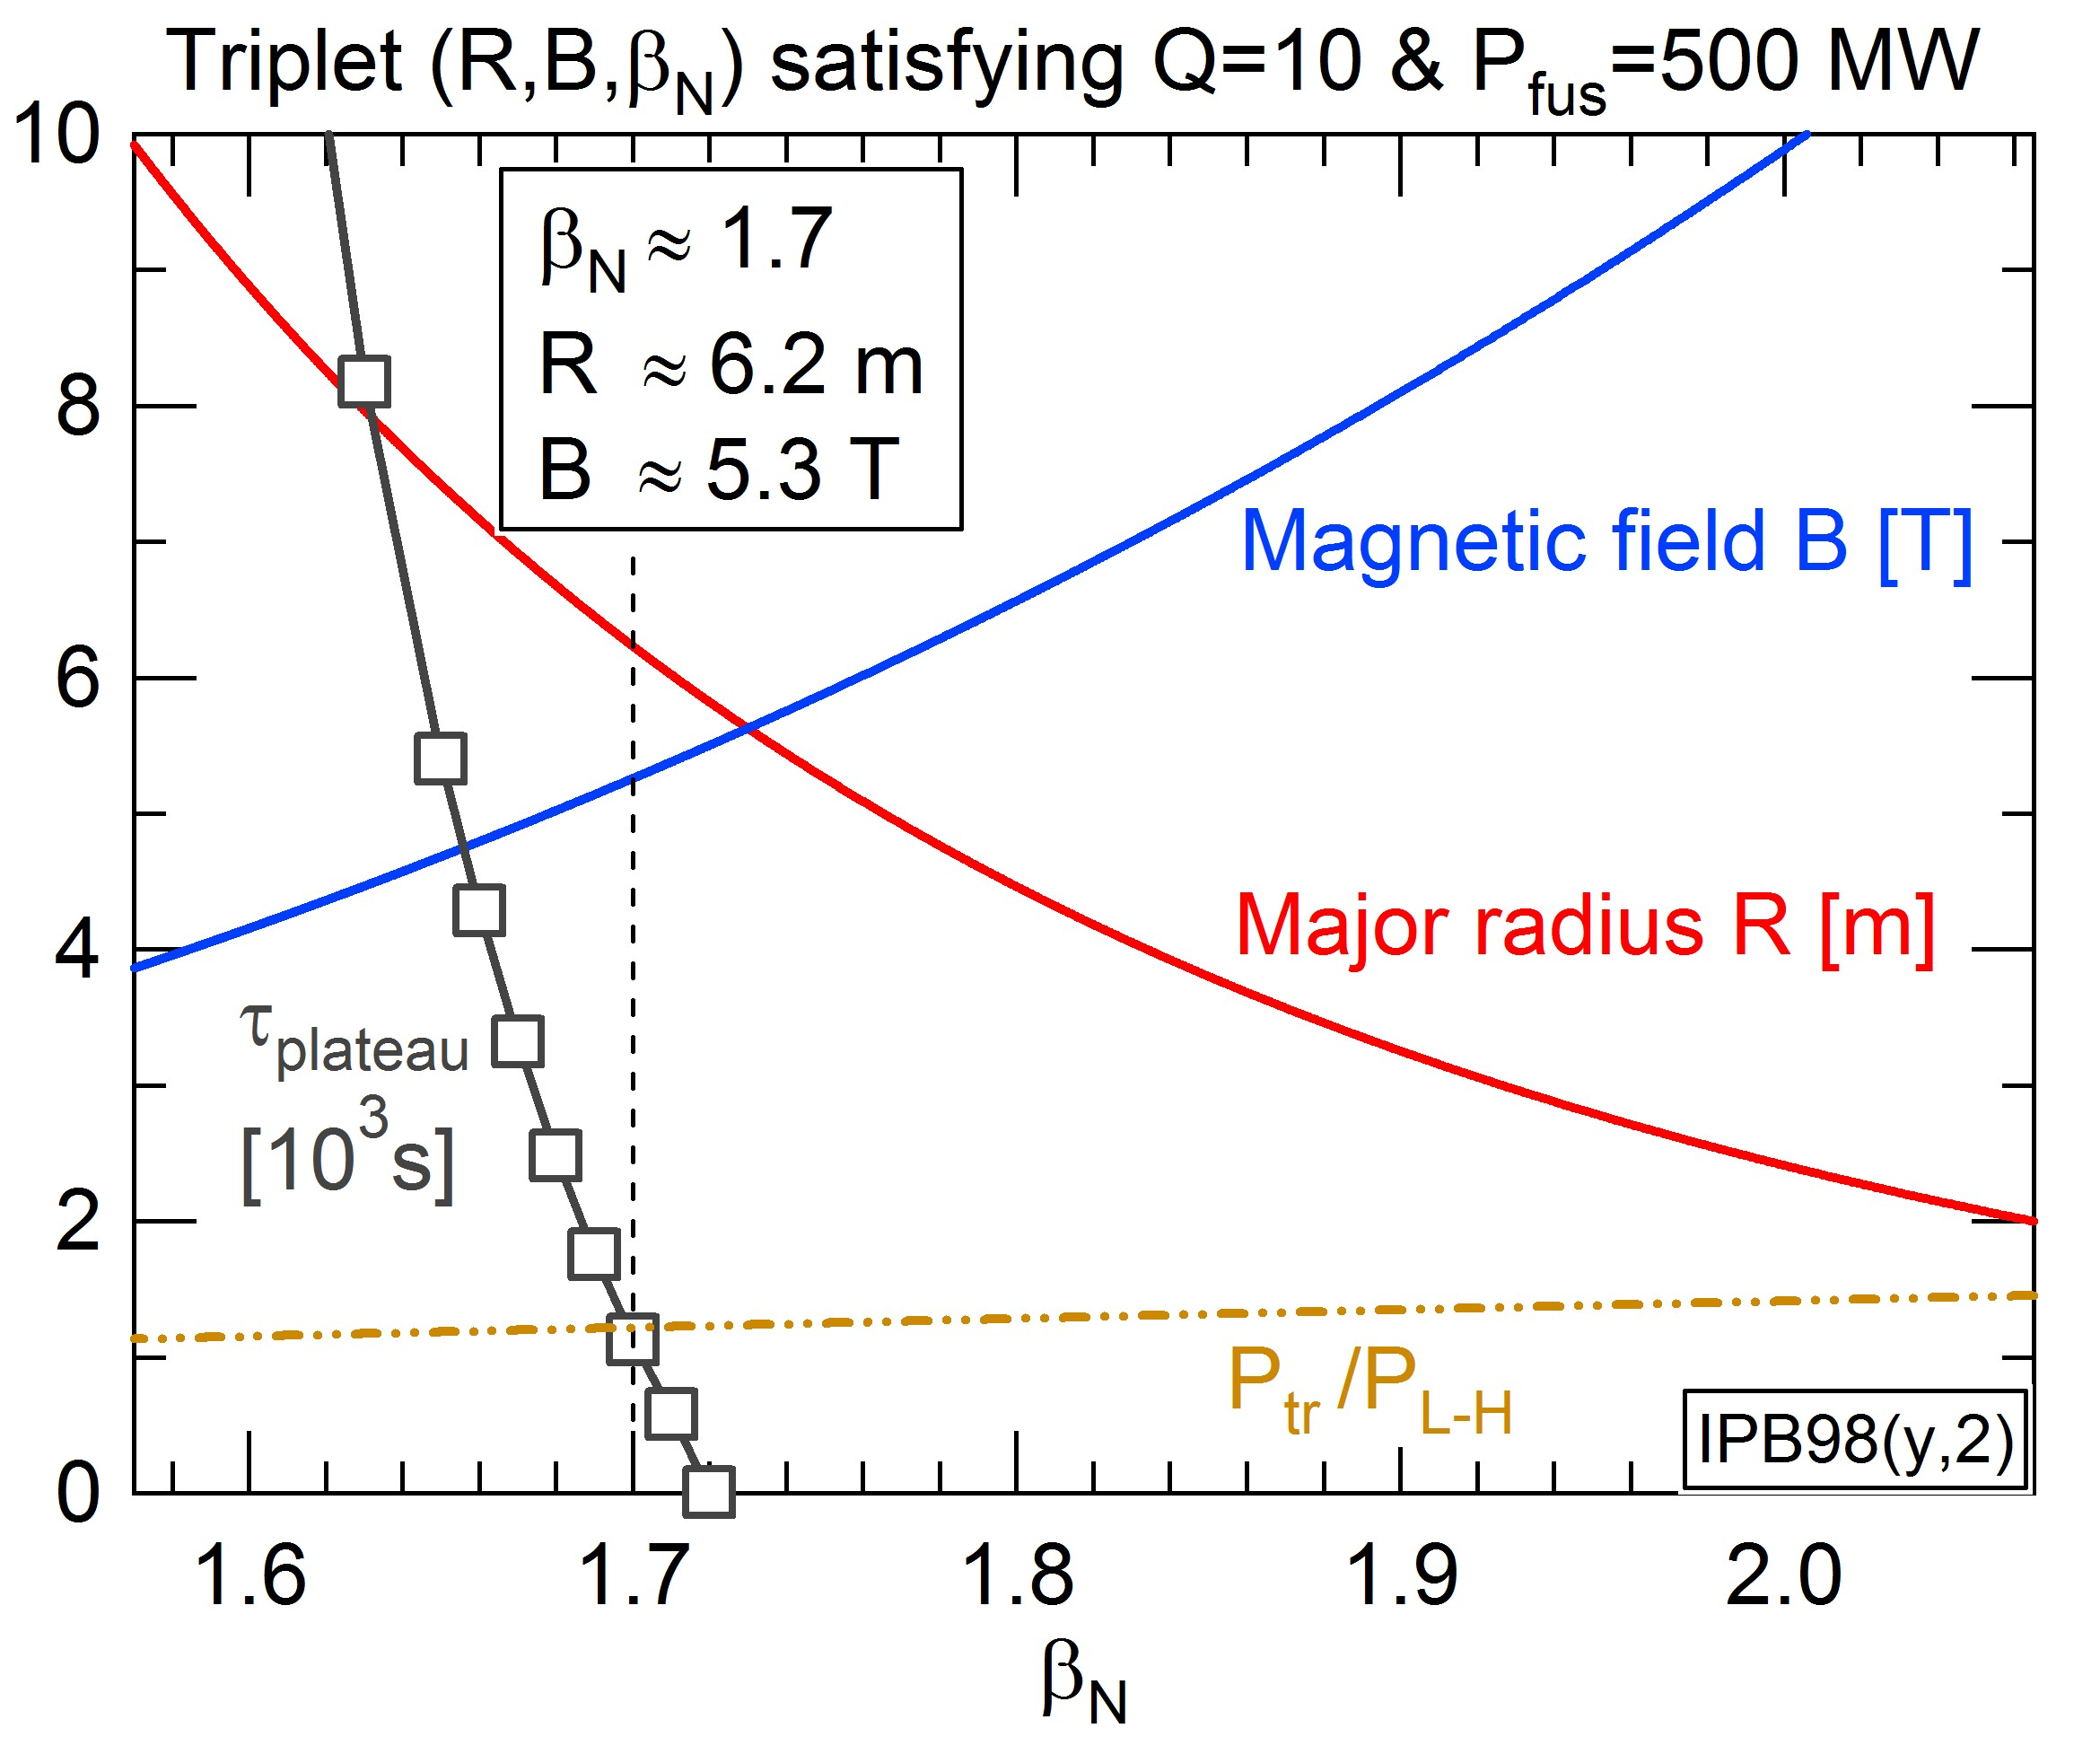
\includegraphics[width=0.55\textwidth]{ITER_IPB98_betaN_R_B.jpg}
	\end{center}
	\caption{Values of $R$ and $B$ as a function of $\beta_N$ which fulfill both equations (\ref{eq:DT_fusion_power_betaN}) and (\ref{eq:nTtau}) when using the IPB98(y,2) scaling law. The solution at $\beta_N \approx 1.7$ is close to the ITER specifications $R_{ITER}=6.2$m, $B_{ITER}=5.3$T. \newstuff{The plasma is supposed to be in H-mode if the ratio $P_{tr}/P_{L-H}$ (see text for definitions) is above unity. } The plateau duration $\tau_{plateau}$ is discussed in section \ref{subsec:radial_build}.}
	\label{fig:solutions_betaN}
\end{figure}

\begin{figure}[htbp]
	\begin{center}
		%\includegraphics[width=0.35\textwidth]{Fig_ITER_IPB98_n_T_Ip_tauE.png}
		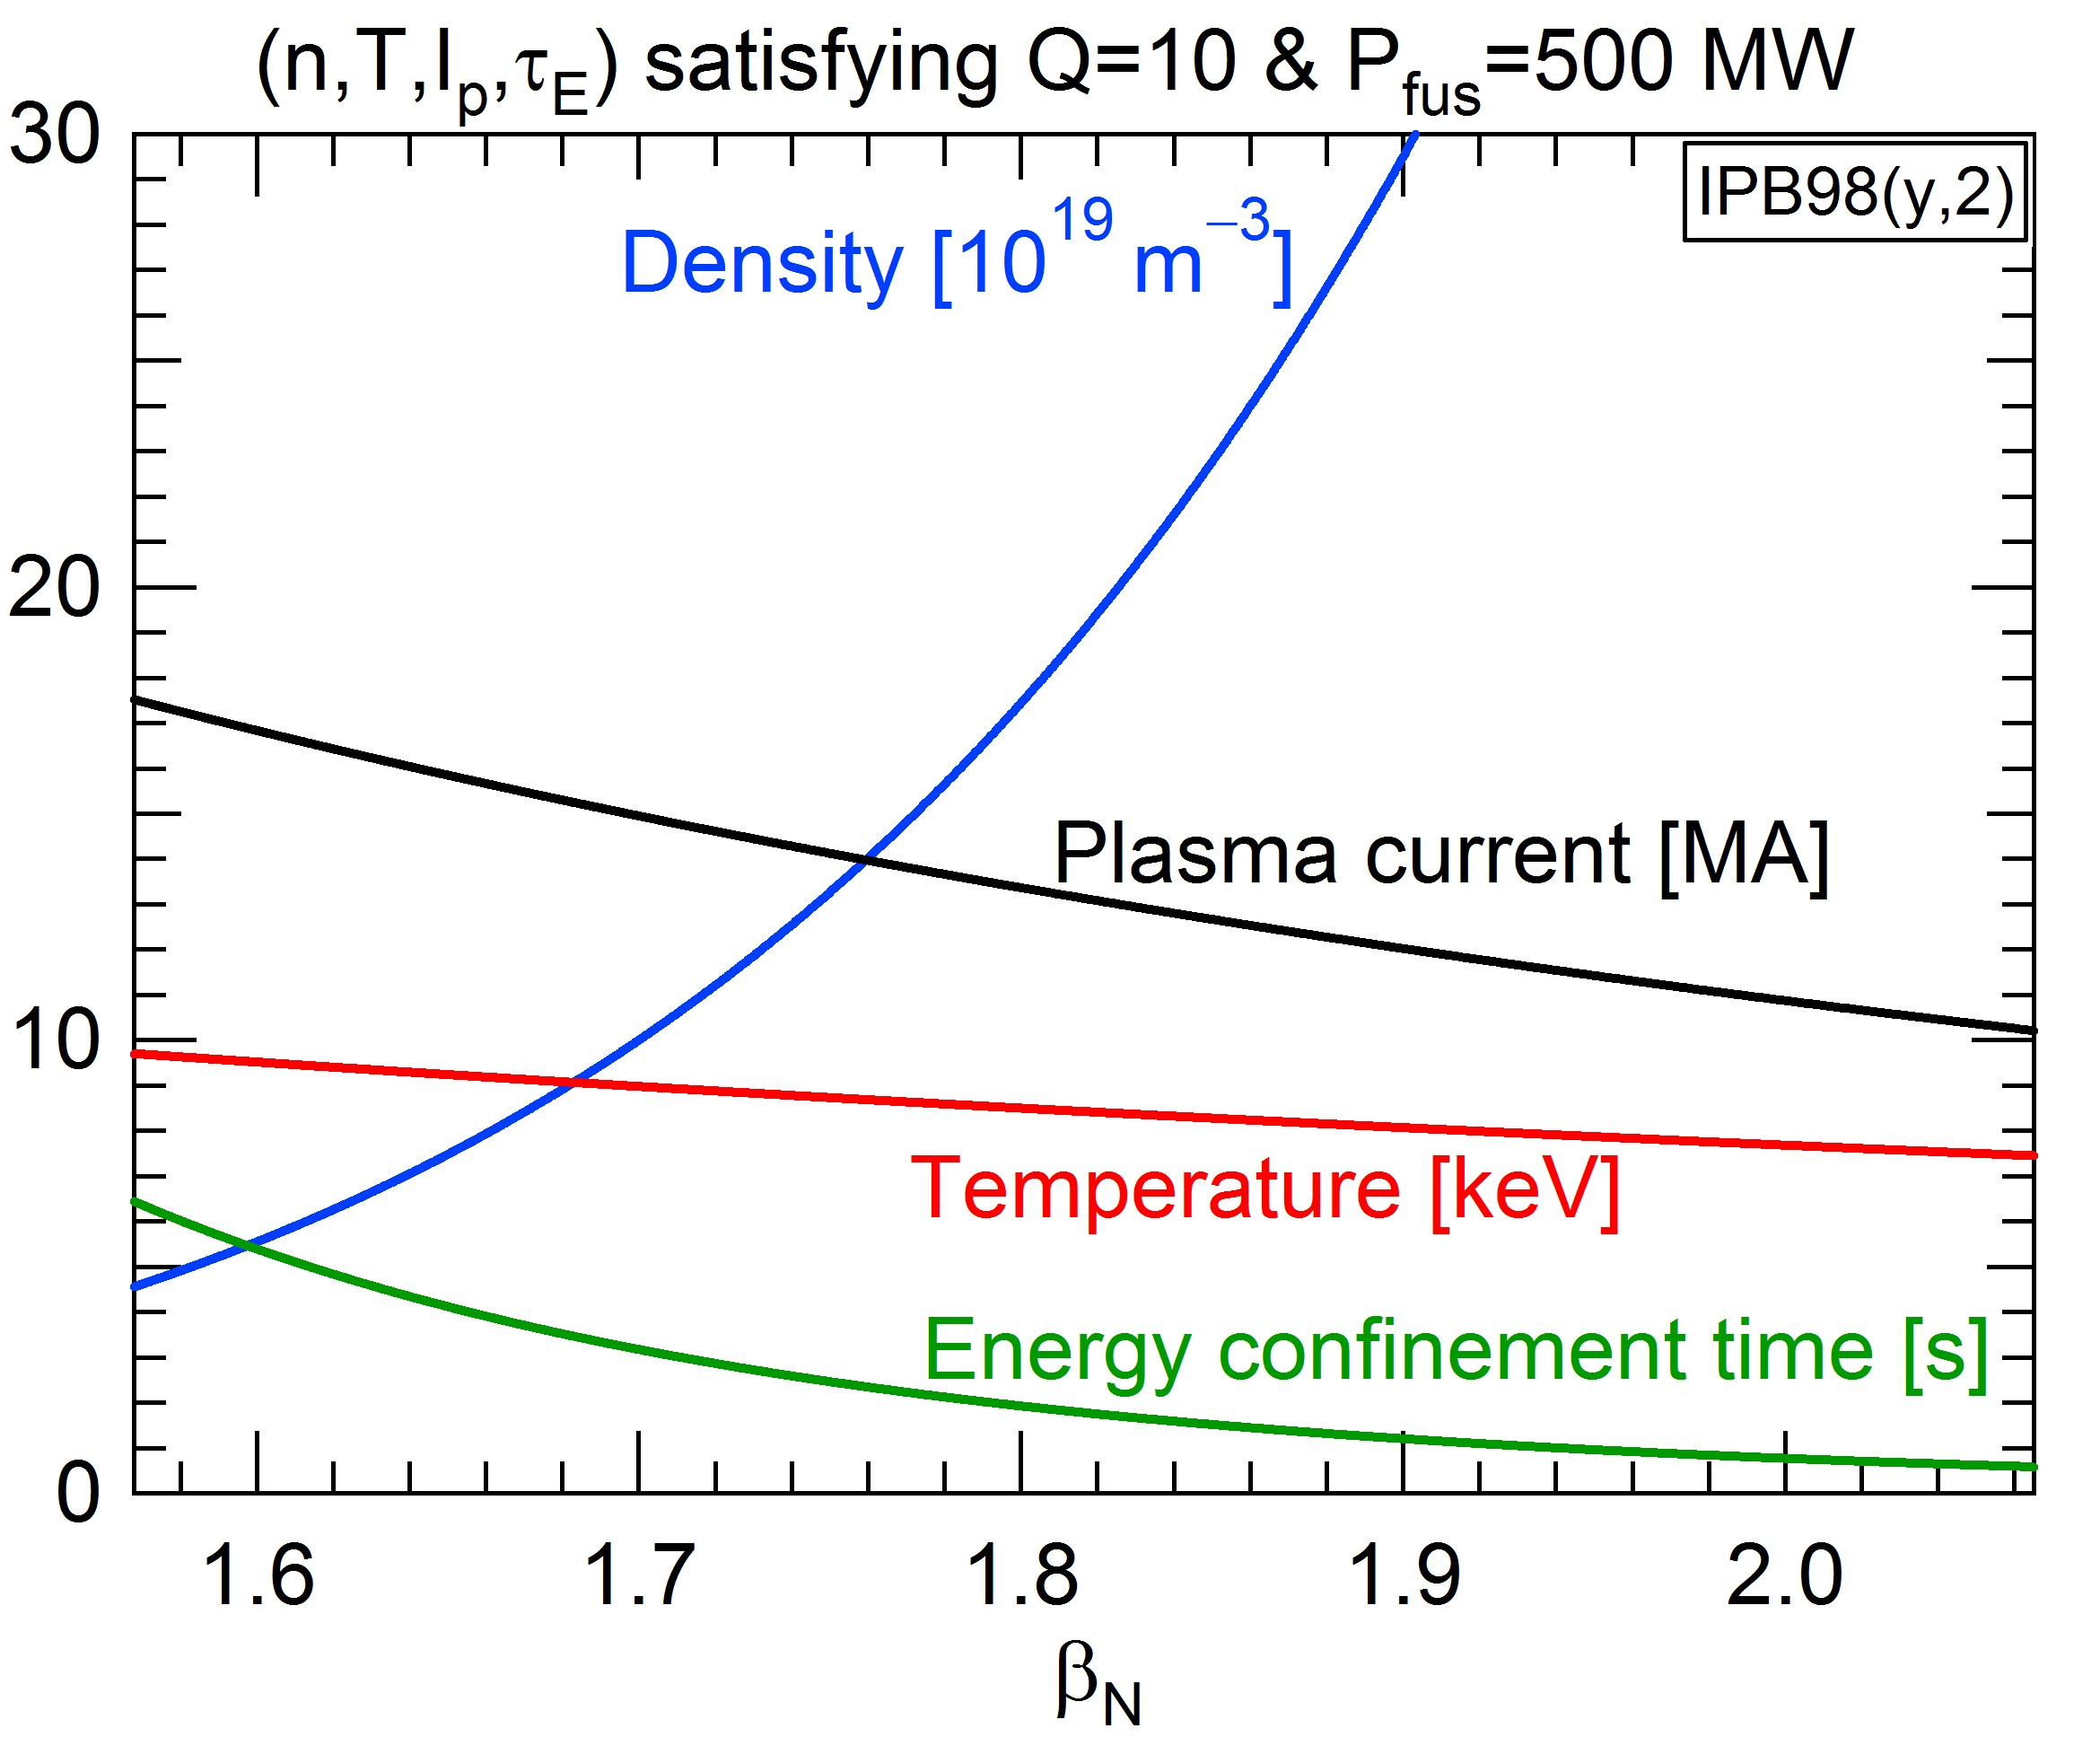
\includegraphics[width=0.55\textwidth]{ITER_IPB98_betaN_n_T_Ip_tauE.jpg}
	\end{center}
	\caption{Normalized density, temperature, plasma current and energy confinement time associated to the $(R,B)$ couples of figure \ref{fig:solutions_betaN}. The dashed horizontal lines correspond to the interval of temperatures where $\langle \sigma v \rangle$ scales like $T^2$.}
	\label{fig:nTIp_IPB98}
\end{figure}

For each triplet, the other physical variables can be calculated from the previous relations:
\begin{eqnarray*}
	\widehat I_p &=& C_I \varepsilon^2 \frac{RB}{q} \\
	\widehat n &=& C_nC_I \frac{B\; n_N}{qR}\\ 
	\widehat T &=& \frac{\varepsilon}{C_nC_\beta} \frac{RB\beta_N}{n_N} \\
%	\widehat W &\doteq& C_{tr}\; \kappa \varepsilon^2  \widehat n \widehat T R^3 = \frac{C_{tr}C_I}{C_\beta} \kappa \varepsilon^3 \frac{\beta_N B^2 R^3}{q}
    \tau_E &=& \frac{C_{tr}C_\beta}{\gamma_{rad}C_{fus}C_I} \frac{Q}{1+Q/\lambda} 
     \frac{q}{\varepsilon \beta_N B^2}
\end{eqnarray*}
These values are displayed on figure \ref{fig:nTIp_IPB98}. Density exhibits the largest variations. It increases with $\beta_N$ while temperature and current decrease. Notice that $T$ is always close to the domain of validity of our analysis, i.e. $10.3 < \widehat T < 18.5$. The error regarding the estimate of the D-T fusion rate $\langle \sigma v \rangle$ keeps typically below $10\%$ for temperatures above $\sim 9.3\,$keV and below $\sim 19.2\,$keV.

Interestingly, it appears that the triplet $(R,B,\beta_N) = (6.2\,$m$, 5.3\,$T$, 1.7)$ is a possible solution of the problem. This set of parameters is consistent with ITER specifications. In this case, density, temperature, current and confinement time are also in fair agreement with published values: $n \approx 1.01\; 10^{20}\,$m$^{-3}$, $T \approx 9.0\,$keV, $I_p \approx 14.9\,$MA and $\tau_E \approx 3.1\,$s. 
Also, the heat power crossing the separatrix amounts to about $\widehat P_{tr} \approx 106\,$MW, well above the L-H power threshold of $\newstuff{\widehat P_{L-H}}\sim 87\,$MW estimated from the empirical scaling law of reference \cite{Martin2008} \newstuff{(cf. dashed-dotted line on figure \ref{fig:solutions_betaN})}. Finally, assuming an e-folding length of the heat flux $\lambda_q \approx 5.10^{-3}\,$m in the scrape-off layer, one would expect about $27\,$MW.m$^{-2}$ on the divertor target plates (considering an inclination angle of the tiles of $30^\circ$ and a flux expansion of 5 as commonly retained values). This would require additional radiation at the edge to keep below the technological limit of about $10\,$MW.m$^{-2}$ in steady state. \\

The same exercise is performed when using the zero-$\beta$ DS03 scaling law (see section \ref{subsec:dimensionless} for the definition) proposed in \cite{Sips2018}. The results are displayed on figure \ref{fig:solutions_betaN_Sips2018}, \newstuff{with prescribed parameters given in table \ref{Tab:ITER_parameters}}. The corresponding dimensional variables are plotted on figure \ref{fig:nTIp_Sips2018}. The same trend is observed for $R$ and $B$ with respect to $\beta_N$, but with much larger variations. It readily appears that the ITER specifications are not part of the solutions. One possible choice would be to consider the same radius $R=6.2\,$m, which would then require $B\approx 4.42\,$T and $\beta_N \approx 2.43$ to achieve $Q=10$ and $\hatPfus=500\,$MW.
In this case, density, temperature, plasma current and energy confinement time would be equal to $n \approx 8.4\;10^{19}\,$m$^{-3}$, $T \approx 10.7\,$keV (in between the acceptable limits 10.3 and 18.5), $I_p \approx 12.5\,$MA and $\tau_E \approx 3.1\,$s. Again, the power crossing the separatrix $\widehat P_{tr} \approx 106\,$MW exceeds the L-H power threshold, estimated at $\newstuff{\widehat P_{L-H}}\sim 66\,$MW from \cite{Martin2008}.

\begin{figure}[htbp]
	\begin{center}
		%\includegraphics[width=0.35\textwidth]{Fig_ITER_Sips2018_betaN_R_B.png}
		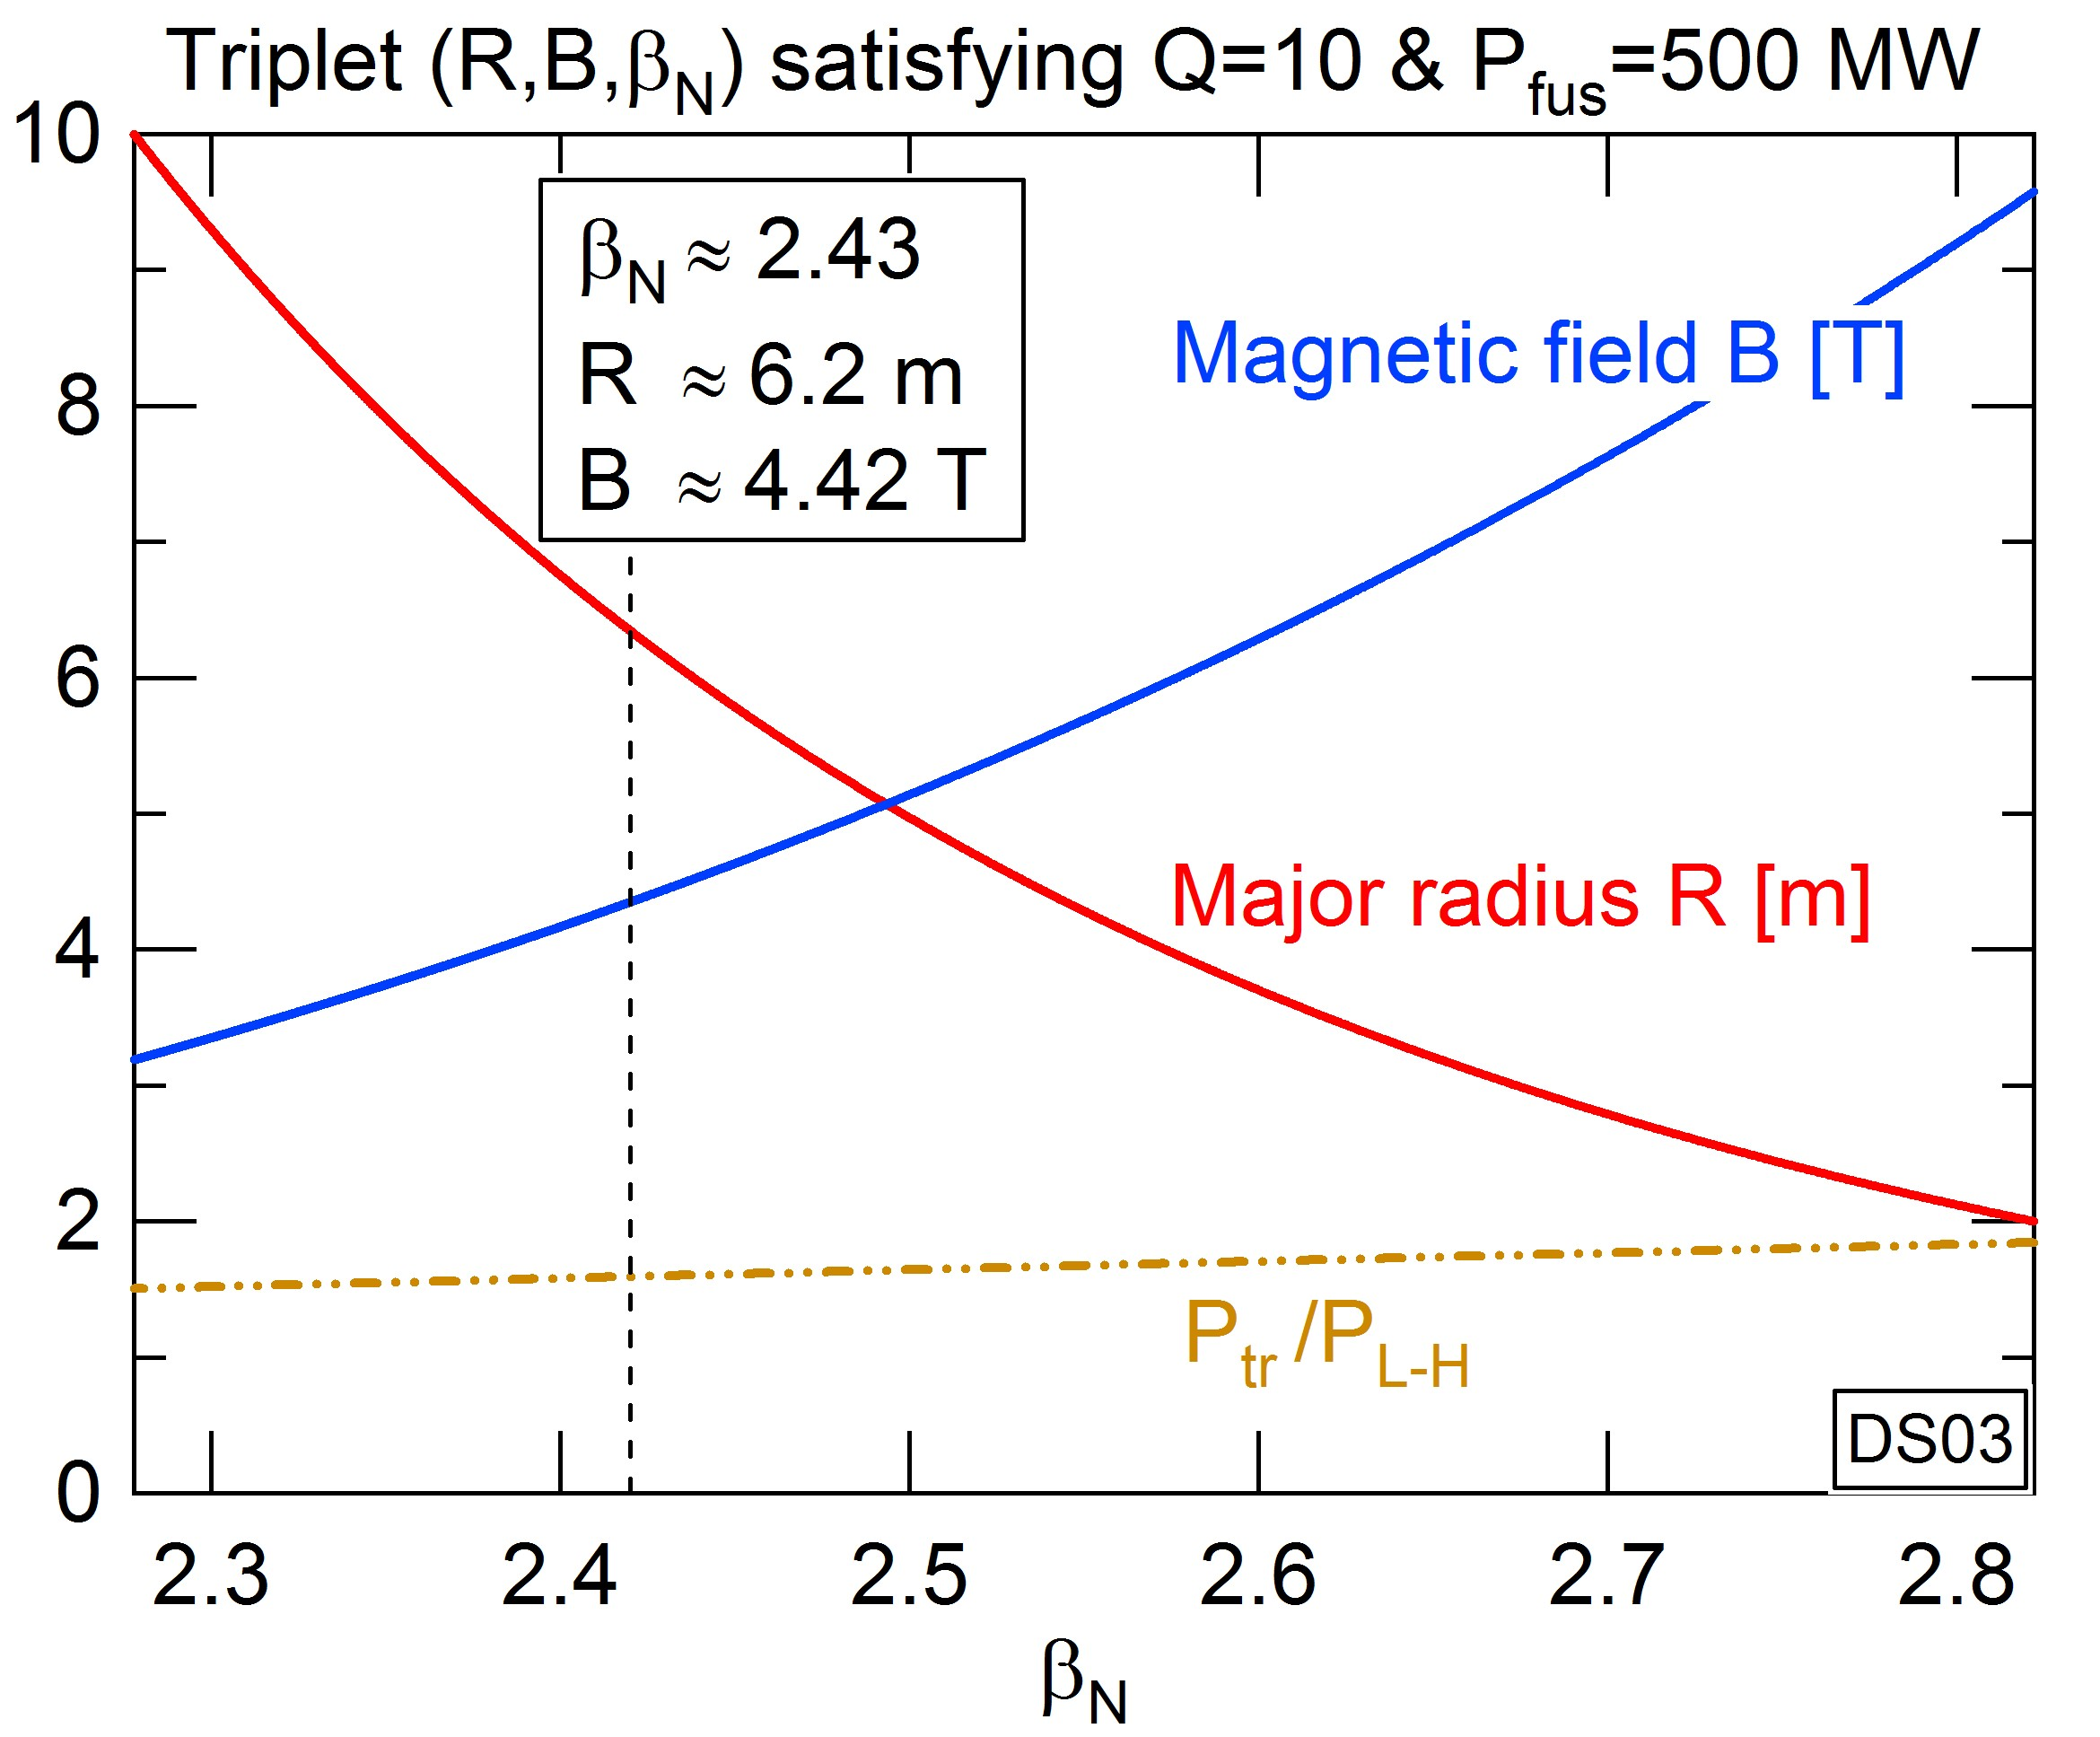
\includegraphics[width=0.55\textwidth]{ITER_DS03_betaN_R_B.jpg}
	\end{center}
	\caption{Same as figure \ref{fig:solutions_betaN} when using the DS03 scaling law \cite{Sips2018}.}
	\label{fig:solutions_betaN_Sips2018}
\end{figure}

\begin{figure}[htbp]
	\begin{center}
		%\includegraphics[width=0.35\textwidth]{Fig_ITER_Sips2018_n_T_Ip_tauE.png}
		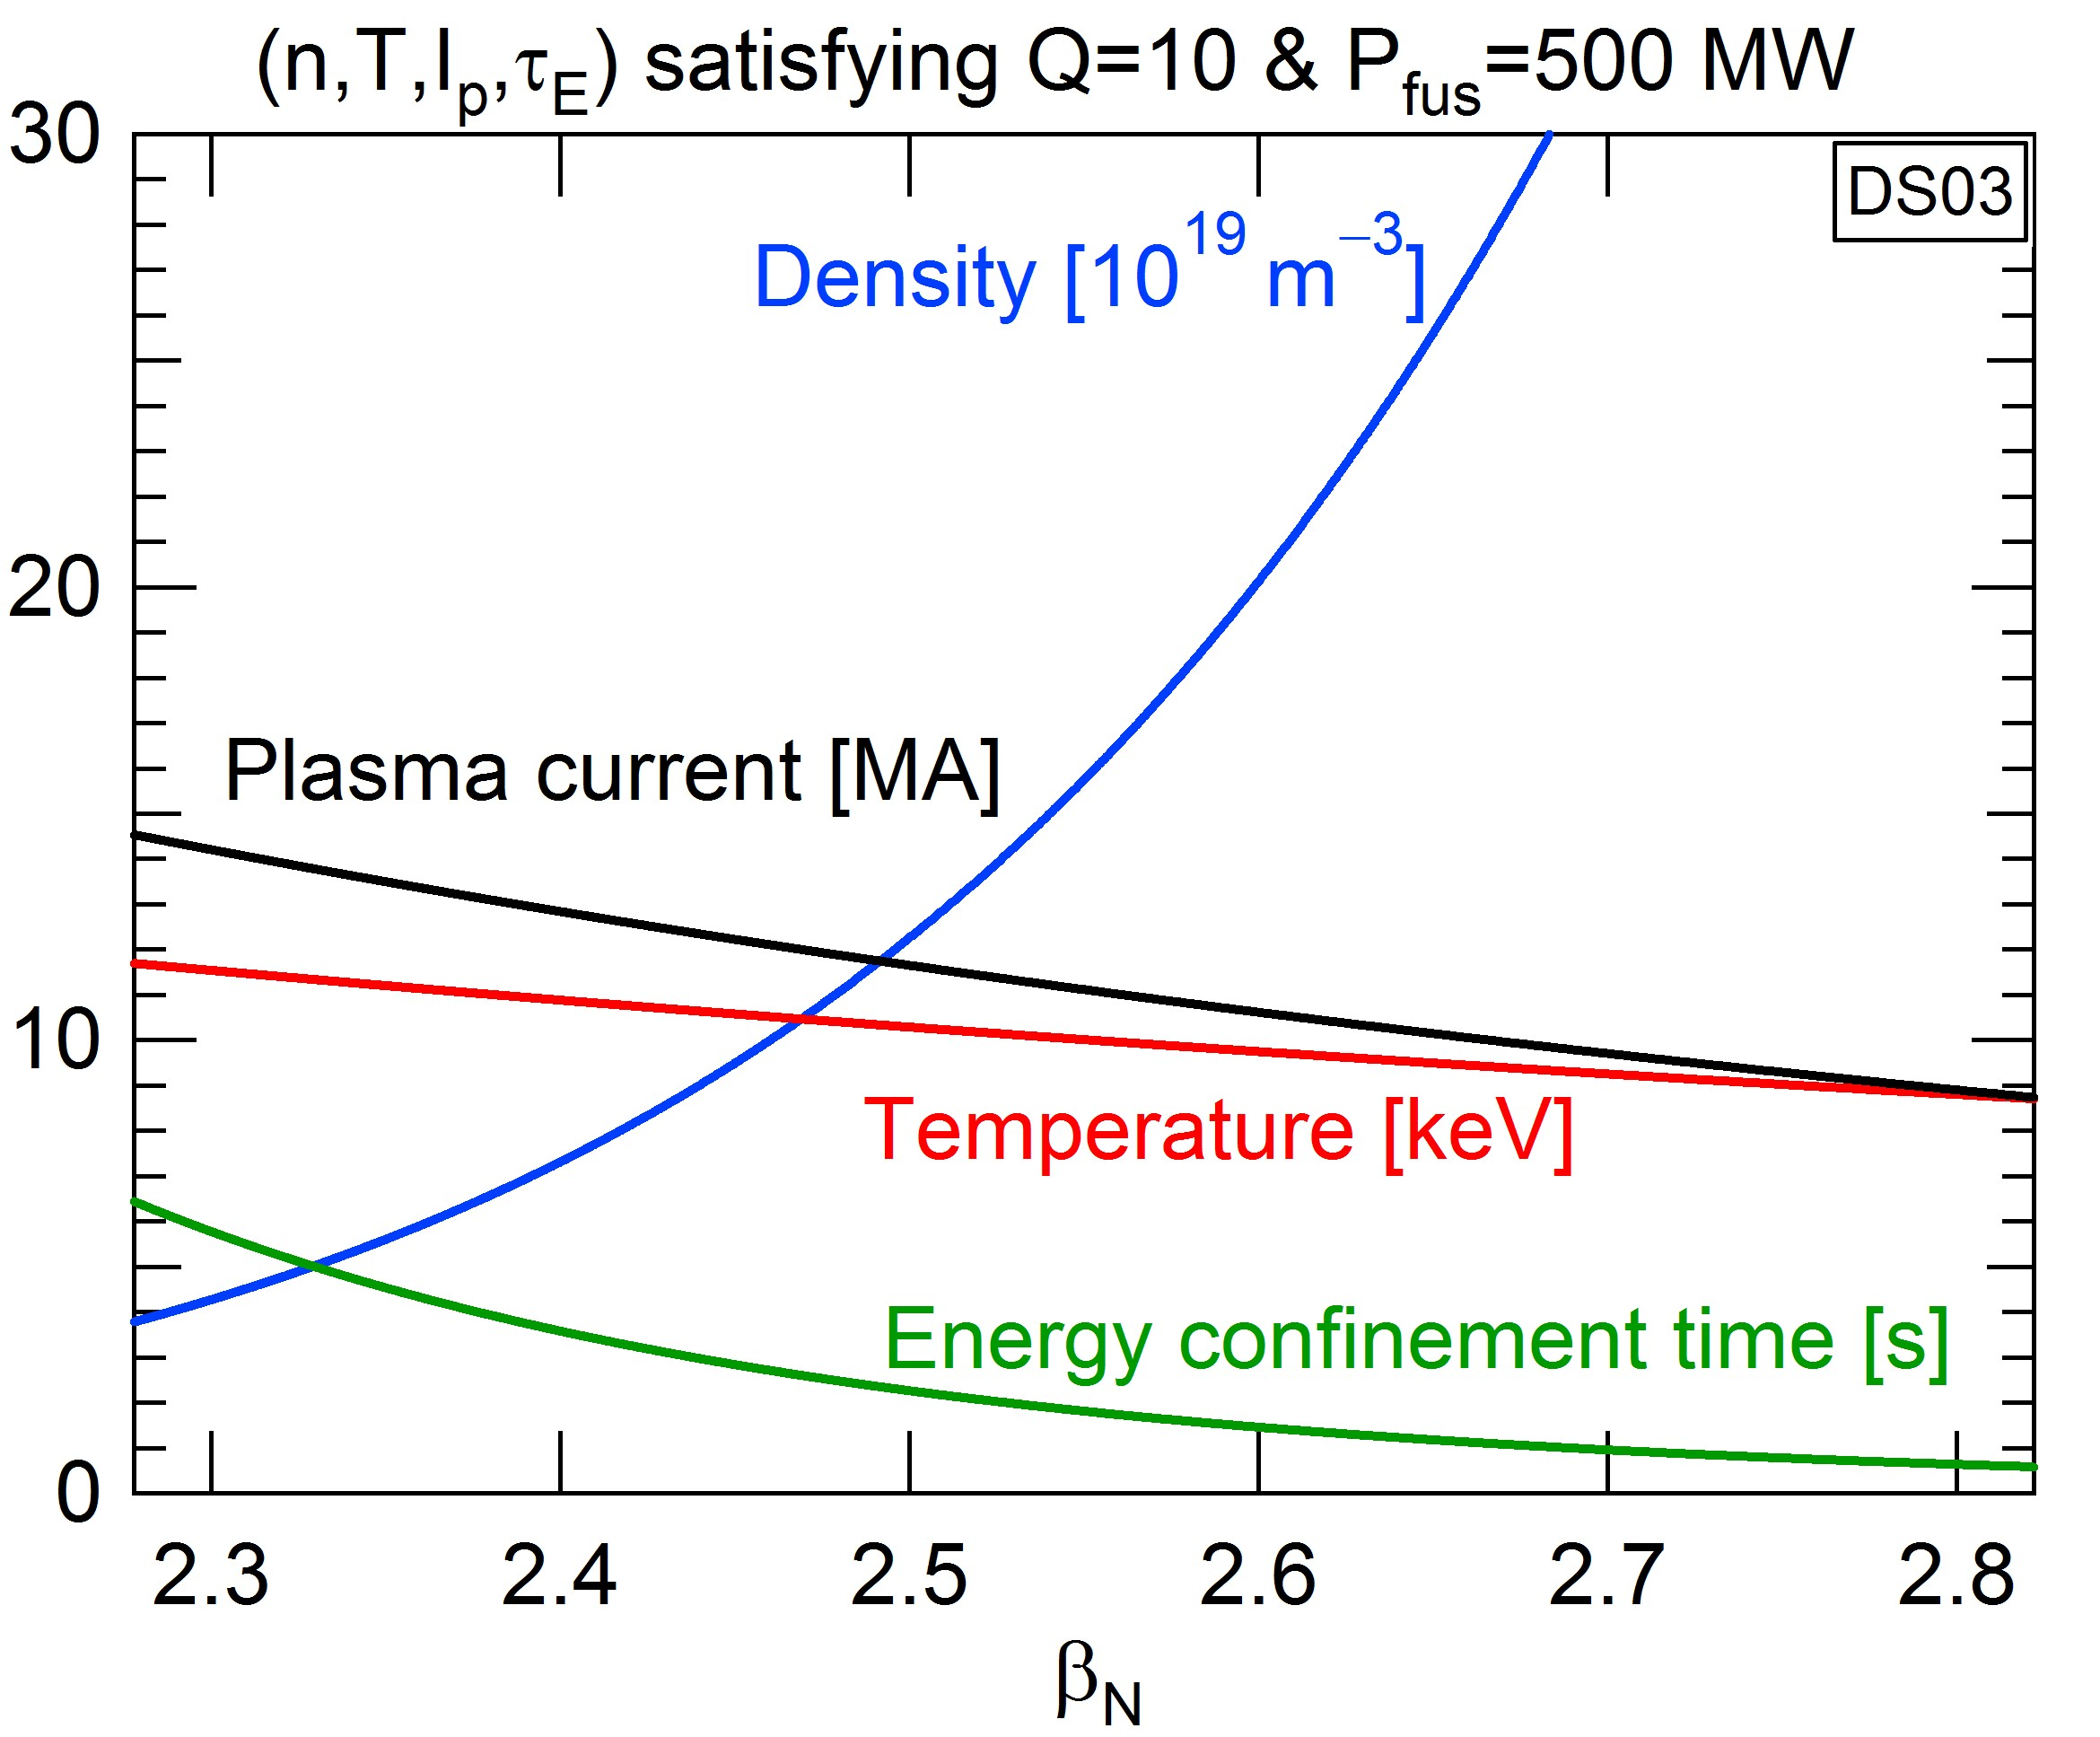
\includegraphics[width=0.55\textwidth]{ITER_DS03_betaN_n_T_Ip_tauE.jpg}
	\end{center}
	\caption{Same as figure \ref{fig:nTIp_IPB98} when using the DS03 scaling law \cite{Sips2018}.}
	\label{fig:nTIp_Sips2018}
\end{figure}


%-------------------------------------------------------------------
\subsection{A word on the engineering constraints} \label{subsec:radial_build}

In addition to scaling laws, there are also engineering constraints in ITER which further shrink the accessible domain for the triplets $(R, B, \beta_N)$ enabling the target $\Pfus$ and $Q$ to be reached (cf. figures \ref{fig:solutions_betaN} and \ref{fig:solutions_betaN_Sips2018}) \cite{Reux2018,Federici2017}. Indeed, one of the critical requirements for ITER deals with the \emph{plateau duration} $\tau_{plateau}$, which measures the time duration during which the discharge achieves its nominal performance in terms of $(\Pfus, Q)$ in \emph{inductive mode}, $i.e.$ such that the plasma current is entirely generated by varying the magnetic flux in the central solenoid.
While this paper mainly focuses on the impact of scaling laws on tokamak dimensioning, it cannot completely ignore the impact of engineering factors. Indeed, as obvious on figure \ref{fig:solutions_betaN}, the risk is otherwise to consider machines which cannot exist in reality, simply because of lack of space inside the inner ring of the torus to put the required materials. 
Actually, these are mostly the blanket, the vacuum vessel and the magnet system which have to be accounted for to constrain the dimensioning, which would otherwise remain virtual. Their radial extension aims at fulfilling the following objectives: respectively ensuring the power extraction, the neutron shielding, the plasma confinement and the magnetic field production required to achieve the target performance in terms of $(\Pfus, Q, \tau_{plateau})$ \cite{Duchateau2014, Federici2017, Reux2018}.  
In a simplified approach, one can assume that the radial extension of the blanket and of the vacuum vessel are known. Then, the radial extension (in the equatorial plane) of the \newstuff{inner legs of the toroidal field coils } and of the central solenoid system are shown to \newstuff{constrain the achievable } $\tau_{plateau}$. Their calculation is detailed in \cite{Duchateau2014}.
The method is applied to the parameters of figure \ref{fig:solutions_betaN}, where the corresponding $\tau_{plateau}$ is plotted (in $10^3\,$s). It appears that, because of the concomitant decrease of $R$ and increase of $B$ with $\beta_N$, the plateau duration $\tau_{plateau}$ exhibits a rapid decay when $\beta_N$ increases. As a matter of fact, the ITER specification imposing $\tau_{plateau} >500\,$s cannot be fulfilled for $\beta_N$ typically larger than 1.7.

%\begin{figure}[htbp]
%	\begin{center}
%		\includegraphics[width=0.45\textwidth]{Fig_tau_plateau.png}
%	\end{center}
%	\caption{Same as figure \ref{fig:solutions_betaN} with the addition of the maximum achievable $\tau_{plateau}$ as a function of $\beta_N$ (see text). ITER specifications impose $\tau_{plateau} >500\,$s.}
%	\label{fig:tau_plateau}
%\end{figure}

%-------------------------------------------------------------------
\subsection{Link with the exponents of dimensionless variables} \label{subsec:dimensionless}

The empirical scaling laws for $\tau_E$ have to exhibit the same scale invariance properties as the underlying equations of the physics at work \cite{Connor1977,Luce2008}. Assuming that quantum physics can be neglected (weak line radiation), one is left with Maxwell and Vlasov (including collisions) equations. Further noticing that core turbulence and transport develop at scales larger than the Debye length, Maxwell-Gauss can be replaced by the quasi-neutrality. On the basis of the pioneering work of Kadomtsev on dimensional analysis in tokamak plasmas \cite{Kadomtsev1975}, one then expects the system to be governed by a reduced set of independent dimensionless parameters, among which $\rho_*$, $\beta$ and $\nu_*$:
\begin{eqnarray}
\rho_*  &\doteq& \lambda_\rho\; \frac{(M \widehat T_i)^{1/2}}{\varepsilon R B} 
\label{eq:rhostar}\\
\nu_*   &\doteq& \frac{qR \varepsilon^{-3/2} \; \nu_{ii}}{(10^3e\, \widehat T_i/M m_p)^{1/2}}
= \lambda_\nu \; 
Z^4 qR \varepsilon^{-3/2}\; \frac{\widehat n}{\widehat T^2} 
\label{eq:nustar} \\
\beta   &\doteq& \lambda_\beta\; \frac{\widehat n\widehat T}{B^2} 
\label{eq:beta}
\end{eqnarray}
with $\lambda_\rho = (2.10^3 m_p/e)^{1/2}$, $\lambda_\nu = 10^{13}\sqrt{\pi}\,e\; \ln\Lambda/(12\pi^2\varepsilon_0^2)$ ($\ln\Lambda$ is the Coulomb logarithm) and $\lambda_\beta = 4.10^{22}e\mu_0$. Here, for the sake of simplicity, $Z$, $\theta_i$ and $f_p$ are taken equal to 1.
Since $\tau_E$ (\ref{eq:tauE_SL_generic_a}) scales with the four dimensional variables $(\widehat n, \widehat T, R, B)$ only (\ref{eq:nTtau_nTRB}), then $\omega_c \tau_E$ is expected to scale with $(\rho_*, \nu_*, \beta)$ only according to \cite{Kadomtsev1975}. Consistently, we shall call this transformation the Kadomtsev transformation. Obviously, because the number of variables reduces from 4 to 3, the power exponent of the fourth variable has to vanish in the transformation; for instance, $\tau_E = G(\widehat n, \widehat T, R, B) \to \omega_c \tau_E = H(\rho_*, \nu_*, \beta, B^0)$, with $\omega_c = eB/(M m_p)$ the ion cyclotron frequency. The constraint of vanishing $B$-exponent is sometimes referred to as the Kadomtsev's constraint \cite{Christiansen1991}. Similarly, recognizing that transport and confinement might not depend on $\beta$, the change of variables would lead to $\tau_E = G(\widehat n, \widehat T, R, B) \to \omega_c \tau_E = H(\rho_*, \nu_*, B^0, R^0)$. This assumption leads to the additional constraint of vanishing $R$-exponent. This constraint turns out to be equivalent to zeroing the scaling exponent of $\beta$ in the aforementioned Kadomtsev transformation, as it should. We shall call this transformation the zero-$\beta$ transformation.

Inverting equations (\ref{eq:rhostar}-\ref{eq:beta}) leads to the following relationships for the Kadomtsev transformation: 
\begin{eqnarray}
 \widehat n &=& \left( B^8\rho_*^2\nu_*^2\beta^3 \right)^{1/5}
 \left( \lambda_\rho^2\lambda_\nu^2\lambda_\beta^3 \frac{q^2 M}{\varepsilon^5} \right)^{-1/5}
 \label{eq:n_rho_nu_beta} \\
 \widehat T &=& \left( \frac{B\beta}{\rho_*\nu_*} \right)^{2/5}
 \left(\frac{\lambda_\rho\lambda_\nu}{\lambda_\beta} 
 \frac{q M^{1/2}}{\varepsilon^{5/2}} \right)^{2/5}
 \label{eq:T_rho_nu_beta} \\
 R &=& \left( \frac{\beta}{\rho_*^6\nu_*B^4} \right)^{1/5}
 \left(\frac{\lambda_\rho^6\lambda_\nu}{\lambda_\beta} 
 \frac{q M^3}{\varepsilon^{15/2}} \right)^{1/5}
 \label{eq:R_rho_nu_beta}
\end{eqnarray}
Injecting these expressions in (\ref{eq:nTtau_nTRB}) -- divided by $\widehat n\widehat T$ and multiplied by $\omega_c$ -- provides the expression of the energy confinement time in dimensionless -- also called ``physics'' -- variables:
\begin{eqnarray}
 \omega_c\tau_E &=& \frac{e}{m_p} 
\frac{\left( C_{SL} C_I^{\alpha_I}C_{tr}^{\alpha_P}\right)^{1/(1+\alpha_P)}}
{\lambda_\rho^{x_\rho} \lambda_\nu^{x_\nu} \lambda_\beta^{x_\beta}} \;
M^{x_M} \kappa^{x_\kappa} \varepsilon^{x_\varepsilon} q^{x_q} \nonumber \\
&& \times  B^{x_B} \rho_*^{x_\rho} \nu_*^{x_\nu} \beta^{x_\beta}
\end{eqnarray}
with 
$x_M = (5\alpha_M+3\alpha_R+3\alpha_I+4\alpha_P-\alpha_n-5)/5(1+\alpha_P)$, 
$x_\kappa = (\alpha_\kappa+\alpha_P)/(1+\alpha_P)$, 
$x_\varepsilon = (2\alpha_\varepsilon+\alpha_I-3\alpha_R-5\alpha_P+2\alpha_n)/2(1+\alpha_P)$, 
$x_q = (-4\alpha_I+\alpha_R+3\alpha_P-2\alpha_n)/5(1+\alpha_P)$, 
$x_\rho = 2(-3\alpha_R-3\alpha_I-9\alpha_P+\alpha_n)/5(1+\alpha_P)$, 
$x_\nu = (-\alpha_R-\alpha_I-3\alpha_P+2\alpha_n)/5(1+\alpha_P)$, 
$x_\beta = (\alpha_R+\alpha_I+8\alpha_P+3\alpha_n)/5(1+\alpha_P)$ and 
$x_B = (5+5\alpha_B-4\alpha_R+\alpha_I+3\alpha_P+8\alpha_n)/5(1+\alpha_P)$.
Kadomtsev constraint imposes $x_B=0$. The zero-$\beta$ scaling further imposes $x_\beta = 0$. This constraint is well fulfilled by the scaling proposed in \cite{Sips2018}, where $x_\beta = 4.4\, 10^{-3}$. The dimensionless coefficients associated to the scaling laws detailed in Table \ref{Tab:scaling_law_coef} are given in Table \ref{Tab:scaling_law_coef_dimensionless}. The last line shows that all three scaling laws fulfill Kadomtsev constraint. Interestingly, also notice that the newly proposed DS03 scaling law for ELMy H-mode plasmas predicts an opposite trend of $\tau_E$ with respect to the aspect ratio: there, $\tau_E$ is expected to significantly increase with the aspect ratio, while the former IPB98(y,2) scaling predicts the opposite. This uncertainty reflects the lack of machines with sufficiently different $\varepsilon$ values, and the likely bias which exists for compact tokamaks, which usually operate at larger $\beta_N$ values than more conventional tokamaks. Forthcoming data from the WEST tokamak, which should operate at large aspect ratio $\varepsilon^{-1} \sim 5$, will likely help alleviating the uncertainty \cite{Bucalossi2011}. The impact of the aspect ratio on the dimensioning of DEMO is discussed in section \ref{subsec:DEMO}, in the light of the inverse trend of the two scaling laws.

It also appears that, because of the effect of the coefficients, certain exponents of the engineering variables play a more critical role than others, in the sense that a weak modification of their value translates into significant changes of the  exponents of dimensionless variables (see also \cite{Ghendrih2014} on this issue). For instance, if the uncertainty on $\alpha_P$ is of the order of $\pm5\%$ (and modifying $\alpha_n$ by less than $\pm3\%$ to preserve Kadomtsev constraint), then $x_\rho$ and $x_\beta$ are modified by about $-4\% \;/ +9\%$ and $+29\% \;/ -56\%$ respectively in the IPB98(y,2) scaling law ($x_\rho$ changes by $-2\% \;/ +3\%$ while $x_\beta$ is no longer vanishing, ranging from $+0.08$ to $-0.08$ in the DS03 scaling law). Since $x_\rho$ and $x_\beta$ significantly impact the dimensioning of tokamaks -- as discussed below, such sensitivities advocate for refined accuracy with respect to the determination of these scaling exponents. \\

\begin{table}
	\caption{\label{Tab:scaling_law_coef_dimensionless} Coefficients of a the scaling laws for $\tau_E$ discussed in Table \ref{Tab:scaling_law_coef} when expressed in dimensionless variables.}
	\begin{indented}
		\item[]\begin{tabular}{@{}lccc}
			\br
			Name & IPB98(y,2) & DS03 & L-mode
			\\ 
			Ref. & \cite[eq.(20)]{ITERphysics_chap2} & \cite{Sips2018} & \cite[eq.(24)]{ITERphysics_chap2}
			\\ \br
			$x_M$ & $0.95$ & $0.81$ & $0.67$ \\ \mr
			$x_\kappa$ & $3.29$ & $2.29$ & $3.22$ \\ \mr 
			$x_\epsilon$ & $0.73$ & $-1.30$ & $0.09$ \\ \mr
			$x_q$ & $-3.00$ & $-1.71$ & $-3.47$ \\ \mr
			$x_\rho$ & $-2.68$ & $-3$ & $-1.85$ \\ \mr 
			$x_\nu$ & $-0.01$ & $-0.14$ & $0.19$ \\ \mr 
			$x_\beta$ & $-0.90$ & $0.00$ & $-1.41$ \\ \mr 
			$x_B$ & $6.4\, 10^{-3}$ & $4.4\, 10^{-3}$ & $0$ \\ \br
		\end{tabular}
	\end{indented}
\end{table}

The objective here is to understand how the major radius scales with the scaling exponents $x_\rho$, $x_\nu$ and $x_\beta$ of the dimensionless variables $\rho_*$, $\nu_*$ and $\beta$, respectively.
Indeed, working with dimensionless variables allows one to explore the impact of modified scaling exponents, since each can be changed independently without affecting the physical consistency of the data. Prescribing $B$ in (\ref{eq:betaN_R_B}-\ref{eq:Q_R_B}) allows one to express $R$ and $\beta_N$ as functions of known variables, i.e. of $(Q, \hatPfus, n_N, B, ...)$. Hereafter, the ITER target values are considered (cf. Table \ref{Tab:ITER_parameters}). In particular, equation  (\ref{eq:Q_R_B}) can be rewritten as follows:
\begin{eqnarray}
  R &=& \left\{ \left( \frac{Q}{\gamma_{rad}(1+Q/\lambda)} \right)^{\ell_Q} 
  \frac{ C_{tr} C_n^{\ell_n} }{ C_{SL} C_I^{\ell_q} C_{fus}^{1/2} }
  \right. \nonumber \\
  &&\left. \times
  \hatPfus^{\ell_P} M^{-\alpha_M}
  \kappa^{1/2-\alpha_\kappa} \varepsilon^{\ell_\varepsilon} 
  q^{\ell_q} \widehat n_N^{\ell_n} B^{\ell_B}
  \right\}^{\ell_R}
\end{eqnarray}
where
$\ell_Q = 5/\sigma$, 
$\ell_q = -\alpha_R+ 5(-3x_\rho +10x_\nu -3x_\beta)/\sigma$, 
$\ell_n = 5(x_\rho/2 -3x_\nu)/\sigma$,
$\ell_P = (\sigma-10)/2\sigma$,
$\ell_\varepsilon = 2\alpha_R-\alpha_\varepsilon + 5(9x_\rho/2 -12x_\nu +5x_\beta+1)/\sigma$,
$\ell_B = 5(3x_\rho/2 -3x_\nu +2x_\beta+1)/\sigma$
and $\ell_R = 2\sigma /[5(-5x_\rho/2 +2x_\nu -3x_\beta -3)]$
with $\sigma = 5(1 -x_\rho/2 +2x_\nu -x_\beta)$.

Keeping the magnetic field constant at $B=5.3\,$T and varying $x_\rho$ from $-3$ to $-2$ -- possibly mimicking the transition from gyroBohm to Bohm transport -- it is found that the major radius increases from $5.3\,$m to $10.5\,$m for the IPB98(y,2) scaling law (and from $4.8\,$m to $22.7\,$m for the DS03 scaling law). The $\rho_*$ parameter almost scales like $1/R$ in this operation. The smaller size which is required at $x_\rho =-3$ to achieve given performance is a consequence of the better confinement which characterizes gyroBohm transport regimes. 

The exponent $x_\beta$ of $\beta$ has been varied from $-1.5$ to $0$. In this case, the major radius decreases from $6.9\,$m to $4.3\,$m for the IPB98(y,2) scaling law (and from $7.9\,$m to $4.8\,$m for the DS03 scaling law). The issue regarding the $\beta$ dependence of the scaling law of the energy confinement time then appears as extremely important for the dimensioning of tokamaks.

Conversely, when varied from $-0.2$ to $+0.2$ (still at constant $B=5.3\,$T), the $x_\nu$ scaling coefficient weakly affects the size of the machine (by less than $3\%$ and less than $19\%$ in this range for the IPB98(y,2) and DS03 scaling laws, respectively).


%-------------------------------------------------------------------
\subsection{Discussion regarding DEMO} \label{subsec:DEMO}

Conversely to ITER, DEMO specifications are not fully settled yet \cite{Zohm2010}. Yet, significant progress have been made \cite{Federici2017}, putting much emphasis on the impact of current uncertainties on the strategical choices \cite{Coleman2016, Coleman2019}. For the purpose of our analysis, we will hereafter prescribe a certain number of parameters within the right range of magnitude corresponding to the DEMO1 design (cf. \cite[Table 1]{Wenninger2017}). Especially, one targets $Q=40$ and $\hatPfus = 2.037\,$GW, hence requiring about $51\,$MW of auxiliary heating. The remaining parameters which are considered hereafter are detailed in Table \ref{Tab:DEMO_parameters}. The numerical values of the corresponding coefficients introduced in section \ref{sec:Key Physics input for reactor design} are given in Table~\ref{Tab:DEMO_coefficients}. Several parameters are changed as compared to ITER. The aspect ratio, the edge safety factor and elongation are about the same. The fraction of $\alpha$ particles is increased up to $10\%$ to account for the expected larger amount of fusion reactions. The temperature peaking factor is increased at $1.5$ for the same reason (this would correspond to $\nu_T\approx 1.41$ with the profile shapes discussed in section \ref{subsec:refined_coefs}). Also, the radiation fraction is increased (lower $\gamma_{rad} =0.56$) to account for larger Bremsstrahlung losses and the need to radiate a significant amount of power at the edge via impurity injection 
\footnote{ \label{footnote_gamma_rad} Notice that, according to \cite{Wenninger2017}, the total radiation power is expected to reach about $66\%$ of the total heating power in DEMO1: $(1-\gamma_{rad}) = P_{rad}/P_{Sce} \approx 306/462$ if neglecting the Ohmic heating power. However, as discussed in \cite{Lux2015}, only a fraction of the total radiated power should be subtracted to the source heating power. This additional ``user defined'' parameter aims at accounting for the fact that scenarios with high core radiation have been explicitly excluded from current scaling laws, as pointed out in \cite{Zohm2013}. The retained value 0.56 of the coefficient is consistent with current estimates for DEMO1.}.
Finally, an additional coefficient is usually introduced: $H$ represents the ratio between the expected energy confinement time and the one deduced from the considered scaling law. $H>1$ for IPB98(y,2) or DS03 scaling laws means better confinement than standard H-mode. In line with published data, we have taken $H=1.1$ 

 \begin{table}
 	\caption{\label{Tab:DEMO_parameters} Typical DEMO parameters considered in the paper.}
 	\begin{indented}
 		\item[]\begin{tabular}{ccccc}
 			\br
 			$q$ & $\varepsilon^{-1}$ & $\kappa$ & $\delta$ & $n_N$ \\
 			\mr
 			$3.2$   & $3.1$ & $1.59$ & $0.33$ & $1.2$ \\
 			\br	
 			$f_\alpha$ & $M$ & $f_p$ & $\theta_i$ & $\gamma_{rad}$ \\
 			\mr
 			$0.10$ & $2.67$ & $1.5$ & $1/1.1$ & $0.56$ \\
 			\br
 		\end{tabular}
 	\end{indented}
 \end{table}

 \begin{table}
 	\caption{\label{Tab:DEMO_coefficients} Numerical values of the coefficients introduced in section \ref{sec:Key Physics input for reactor design}.}
 	\begin{indented}
 		\item[]\begin{tabular}{ccccc}
 			\br
 			$C_n$ & $C_I$ & $C_\beta$ & $C_{tr}$ & $C_{fus}$ \\
 			\mr
 			$ 3.183$ & $ 11.873$ & $ 0.732$ & $ 0.086$ & $ 1.30\, 10^{-3}$ \\
 			\br	
 		\end{tabular}
 	\end{indented}
 \end{table}

\begin{figure}[htbp]
	\begin{center}
		%\includegraphics[width=0.48\textwidth]{Fig_DEMO_IPB98_Sips2018_betaN_R_B.png}
		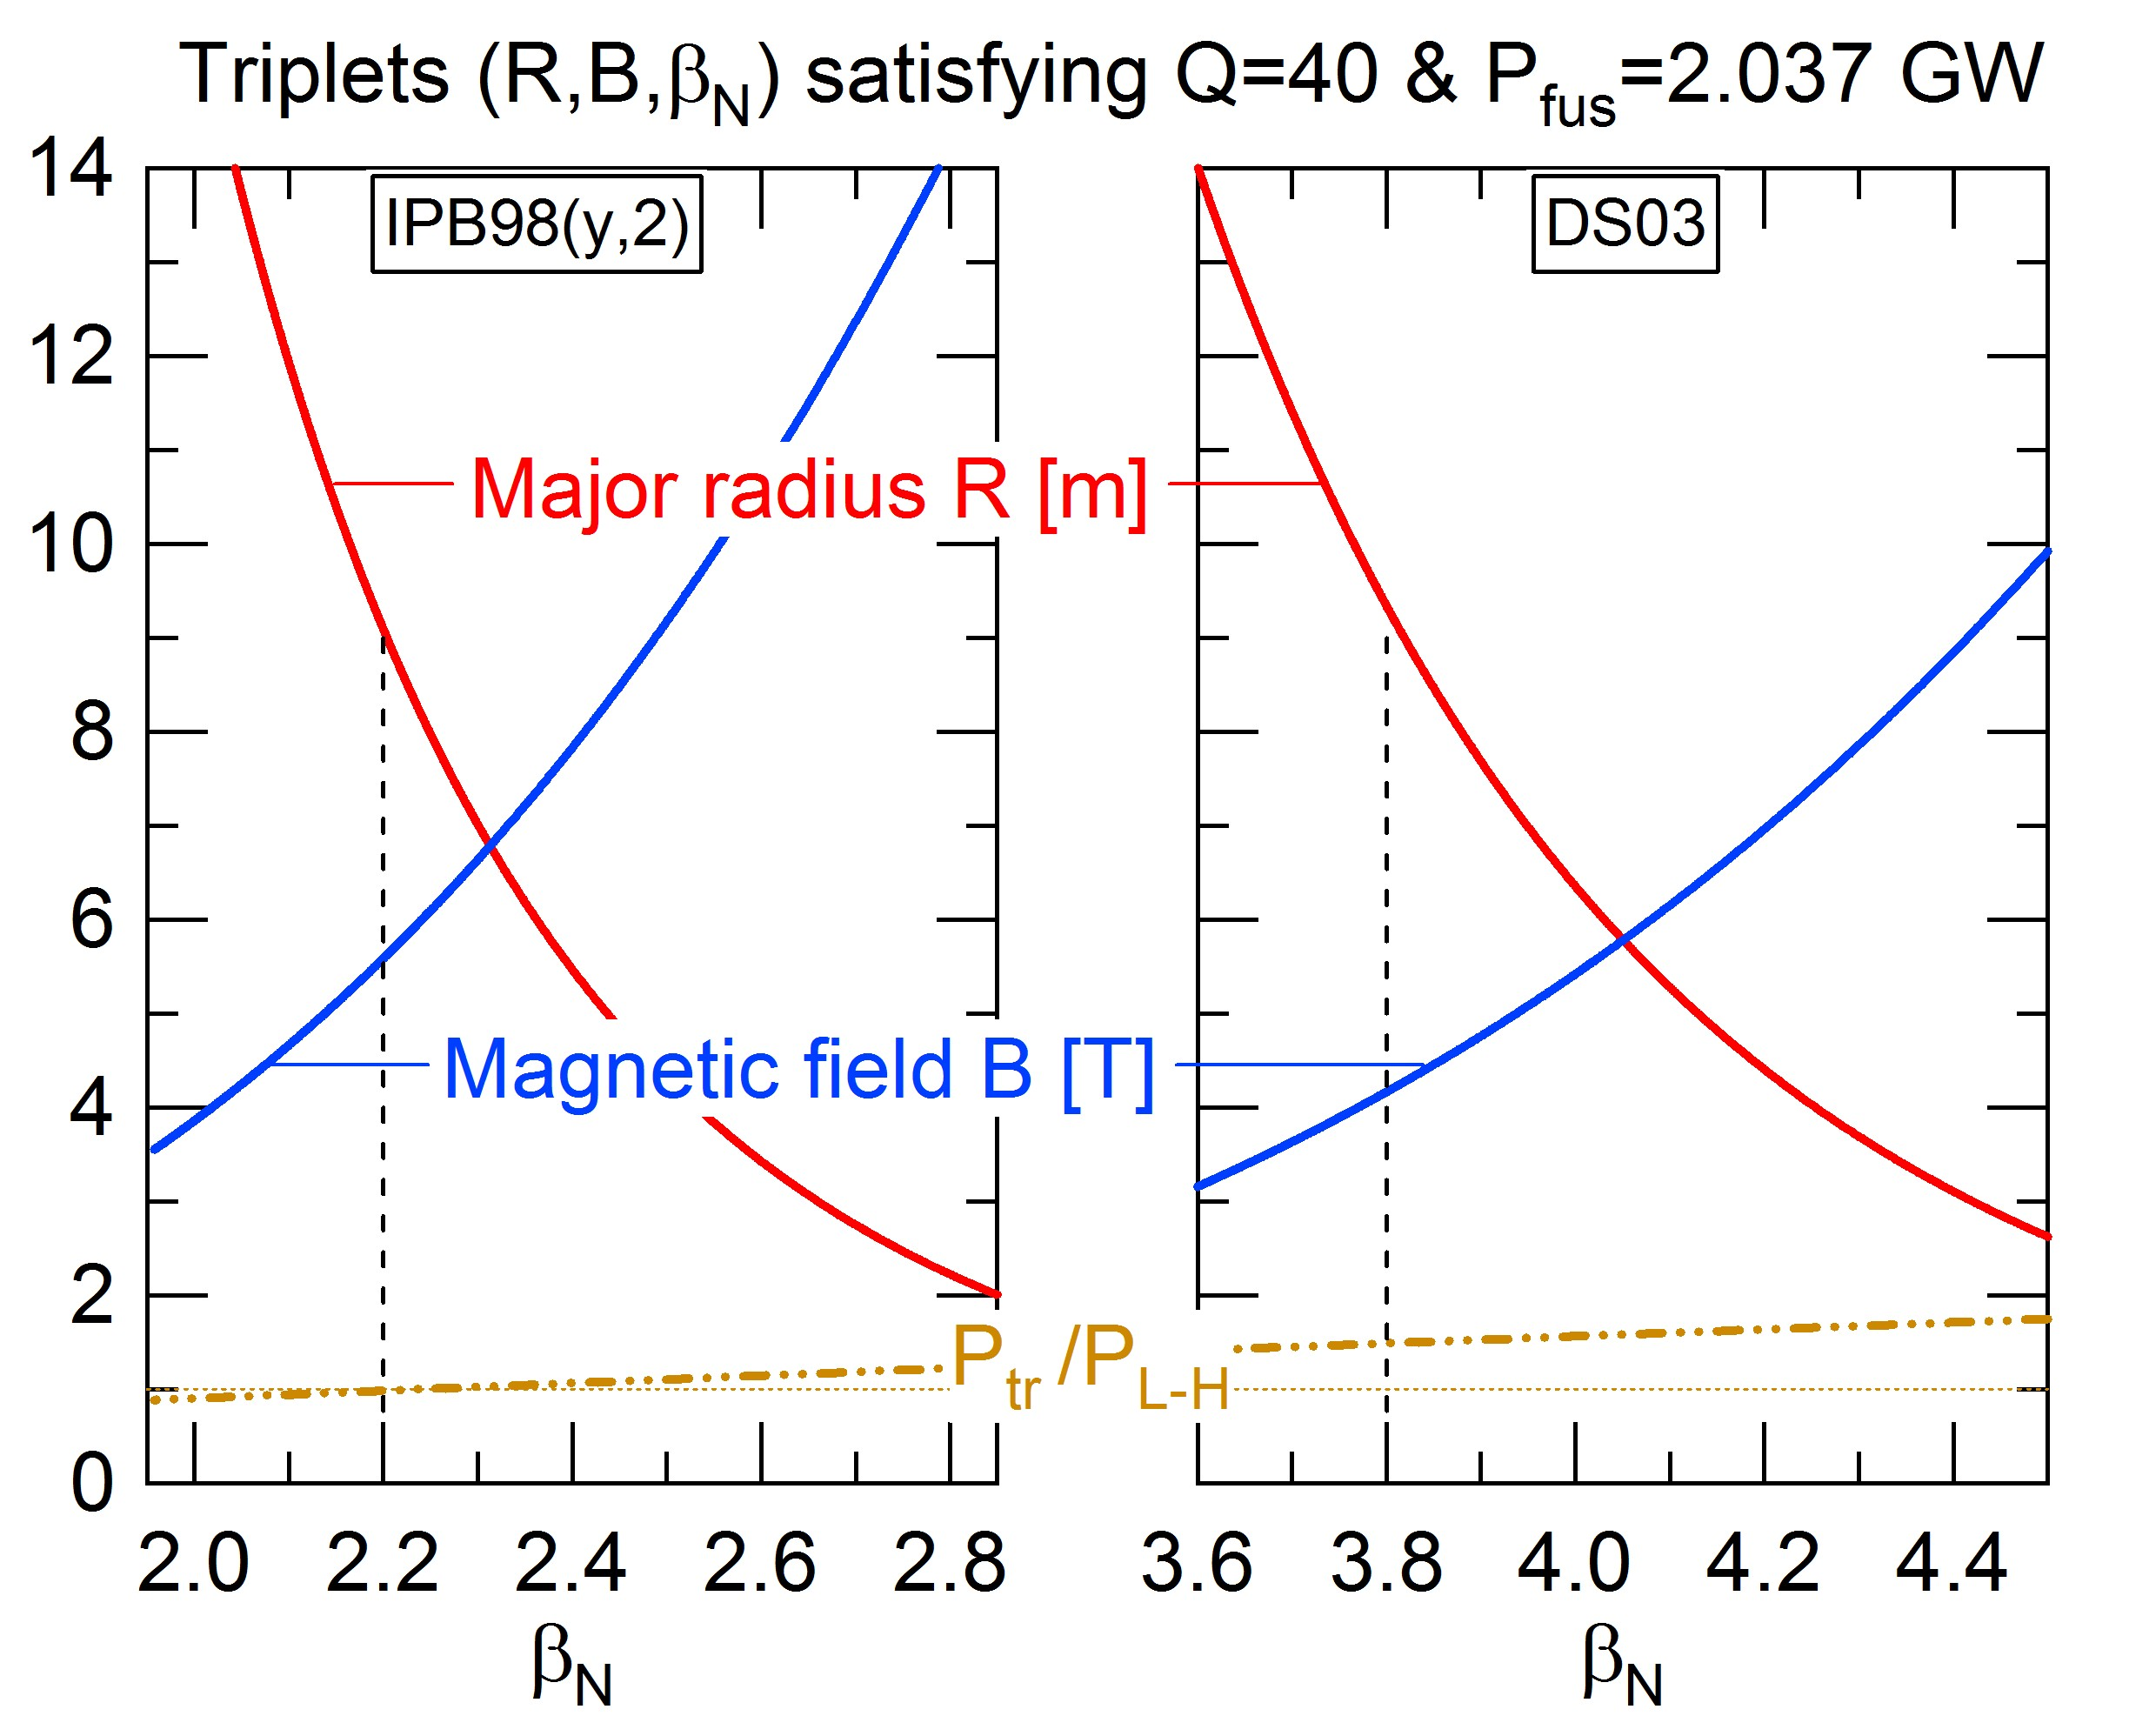
\includegraphics[width=0.75\textwidth]{Layout_DEMO_scan_betaN.jpg}
	\end{center}
	\caption{Same as figure \ref{fig:solutions_betaN} for DEMO specifications \newstuff{(here, $P_{tr}$ is calculated by assuming that 66$\%$ of the heating source is radiated, cf. text)}. Both IPB98(y,2) and DS03 scaling laws are considered.}
	\label{fig:solutions_Hmode_DEMO}
\end{figure}

The solution triplet $(R,B,\beta_N)$ is plotted on figure \ref{fig:solutions_Hmode_DEMO} when considering the two scaling laws for ELMy H-modes. \newstuff{Again, we recall that all other parameters but $(R,B,\beta_N)$ are fixed and given in table \ref{Tab:DEMO_parameters}. } It readily appears that they operate in different parameter ranges with respect to $\beta_N$: while the IPB98(y,2) scaling law finds solutions around $\beta_N\sim2.2$, DS03 predicts solutions closer to $\beta_N\sim3.8$. 
\newstuff{
Such large values of $\beta_N$ may actually reveal difficult to achieve. Indeed, deleterious ideal MHD instabilities are expected to develop above $\beta_{N, crit} \approx 3$ \cite{Strait1994}. Also, the growth of resistive wall modes (RWM) can constitute the primary limitation to $\beta_N$ in advanced tokamak plasma experiments. Although possible optimizations (such as plasma shaping) can increase the achievable $\beta_N$, and feedback loops are efficiently developed to control RWM (see e.g. \cite{Garofalo2001}), such scenarios are all the more challenging in a reactor, which should essentially aim at zero disruptions during its lifetime. Yet, apart from $\beta_N$, both scaling laws 
}
predict solutions in the same range of parameters regarding all other variables. Considering $R_{DEMO}=9.1\,$m \cite{Wenninger2017}, critical variables are listed in Table \ref{Tab:DEMO_results} for both scaling laws. The relative differences reach about $27\%$ for the temperature, larger for DS03% (there, $\widehat T$ exceeds the upper limit $18.5\,$keV, so that the fusion rate is overestimated by about $20\%$)
, density and plasma current, both smaller for DS03. This latter point, and the fact also that $B$ is reduced, make the predictions relying on DS03 more favorable. 
Computing the thermal heat power crossing the separatrix is not an easy task. Indeed, it would require subtracting the entire radiated power inside the separatrix, which is larger than $(1-\gamma_{rad})P_{Sce}$ as discussed above. Considering that it reaches about $66\%$ of the heating source as in \cite{Wenninger2017}, one finds that this power is roughly $\newstuff{P_{tr}\approx} 157.5\,$MW in both cases. \newstuff{Its ratio with respect to the L-H power threshold, $P_{tr}/P_{L-H}$, is plotted on figure \ref{fig:solutions_Hmode_DEMO} (dashed-dotted lines). At $R_{DEMO}=9.1\,$m, $P_{tr}$ exceeds $P_{L-H}$ by about $50\%$ if DS03 holds. Conversely the ratio marginally reaches unity for IPB98(y,2). This may have tremendous consequences regarding technological constraints. Indeed, }one would expect about $27.5\,$MW.m$^{-2}$ on the divertor target plates (with the same assumptions as those for ITER, section~\ref{subsec:ITER_characteristics}), implying the need for additional radiation at the edge \newstuff{to remain below the upper bound of $10\,$MW.m$^{-2}$. Then, given the absence of margin regarding the L-H power threshold, it may actually reveal impossible to fulfill this constraint while still being in H-mode if the IPB98(y,2) scaling law holds (unless relying on the possible hysteresis of the L-H power threshold \cite{Connor2000})}.

Arguing that DEMO cannot face any ELM so as to ensure the safety of its divertor, one might wonder what dimensioning one would expect if operating in L-mode. Using the L-mode scaling law whose coefficients are recalled in Table \ref{Tab:scaling_law_coef}, the model gives the following possible choice for the triplet $(R,B,\beta_N)$: $R\approx 14\,$m, $B\approx 8.9\,$T and $\beta_N \approx0.46$, leading to a heat power crossing the separatrix (same assumption as above) of $\sim 157.5\,$MW below the empirical L-H threshold of $P_{L-H} \sim 535\,$MW. In this case, the required plasma current would be about $47.9\,$MA. In the frame of our simple model, operating DEMO in L-mode looks hardly achievable. \\

\begin{table}
	\caption{\label{Tab:DEMO_results} DEMO characteristic parameters when using IPB98(y,2) and DS03 scaling laws for $\tau_E$.}
	\begin{indented}
		\item[]\begin{tabular}{ccccc} \br
			    & IPB98(y,2) & DS03 \\ \br
			$R_{[m]}$ & $9.1$ & $9.1$ \\ \mr	
			$B_{[T]}$ & $5.6$ & $4.2$ \\ \mr	
			$\beta_N$  & $2.2$ & $3.8$ \\ \mr	
			$\widehat n_{[10^{19}m^{-3}]}$   & $8.7$ & $6.6$ \\ \mr	
			$\widehat T_{[keV]}$   & $12.9$ & $17.0$ \\ \mr	
			$\widehat I_{p\;[MA]}$ & $19.6$ & $14.9$ \\ \mr	
			$\tau_{E\;[s]}$    & $4.6$ & $4.6$ \\ \br
		\end{tabular}
	\end{indented}
\end{table}

As stated in \cite{Wenninger2017}, the aspect ratio $A = R/a$ is a central design parameter in many aspects, including plasma stability issues, disruption forces, tritium breeding, maintenance and cost, among others. Yet, there is some freedom in its choice, although increased stability of divertor detachment regimes -- as required to access strong dissipation of the parallel heat exhaust via efficient radiation -- might favor low aspect ratio machines \cite{Lipschultz2016}. In this framework, and because of the opposite scaling of $\tau_E$ with $\eps$ when expressed in dimensionless variables (cf. section \ref{subsec:dimensionless}), we have explored the sensitivity of the solutions with respect to $A$. For this purpose, fixed values of $\beta_N$ are considered: $\beta_N=2.2$ for the IPB98(y,2) scaling law, and $\beta_N=3.8$ for the DS03 scaling law. The different values account for the different operational spaces for these two scaling laws (cf. figure \ref{fig:solutions_Hmode_DEMO}). The range of variation of $A$ is borrowed from \cite{Wenninger2017}. The results are displayed on figure \ref{fig:solutions_scanA_DEMO}. It readily appears that the variations with $A$ of both solutions $R$ and $B$ are opposite for the two scaling laws. Indeed, while $R$ decreases with $A$ if IPB98(y,2) holds, it increases with $A$ if DS03 holds. The opposite is true for $B$. Besides, the range of variation of $R$ is much larger for DS03 than for IPB98(y,2). \newstuff{Finally, one notices that such scenarios would marginally operate in H-mode for the IPB98(y,2) case ($P_{tr}/P_{L-H}$ ranges from 1.08 at $A=2.6$ down to 0.90 at $A=3.6$ in this case), while the H-mode threshold is well overcome for the DS03 case ($P_{tr}/P_{L-H} \approx 1.67$ at $A=2.6$ and $\approx 1.34$ at $A=3.6$).}

As obvious from this analysis, transport issues, namely scaling laws, may have a strong impact on the final choice of the optimal aspect ratio for DEMO. The two scaling laws which we have considered, although exhibiting roughly the same variance of experimental data (of the order of $16\%$), have opposite signs for the dimensionless scaling exponent of $A=\eps^{-1}$ (see table \ref{Tab:scaling_law_coef_dimensionless}). As a result, they lead to opposite trends for $R$ and $B$ when $A$ is varied at constant $\beta_N$. Consolidating the sign of this exponent, on the basis of both first principle simulations and of novel experiments, appears highly desirable.

\begin{figure}[htbp]
	\begin{center}
		%\includegraphics[width=0.35\textwidth]{Fig_DEMO_scanA_fixed_betaN.png}
		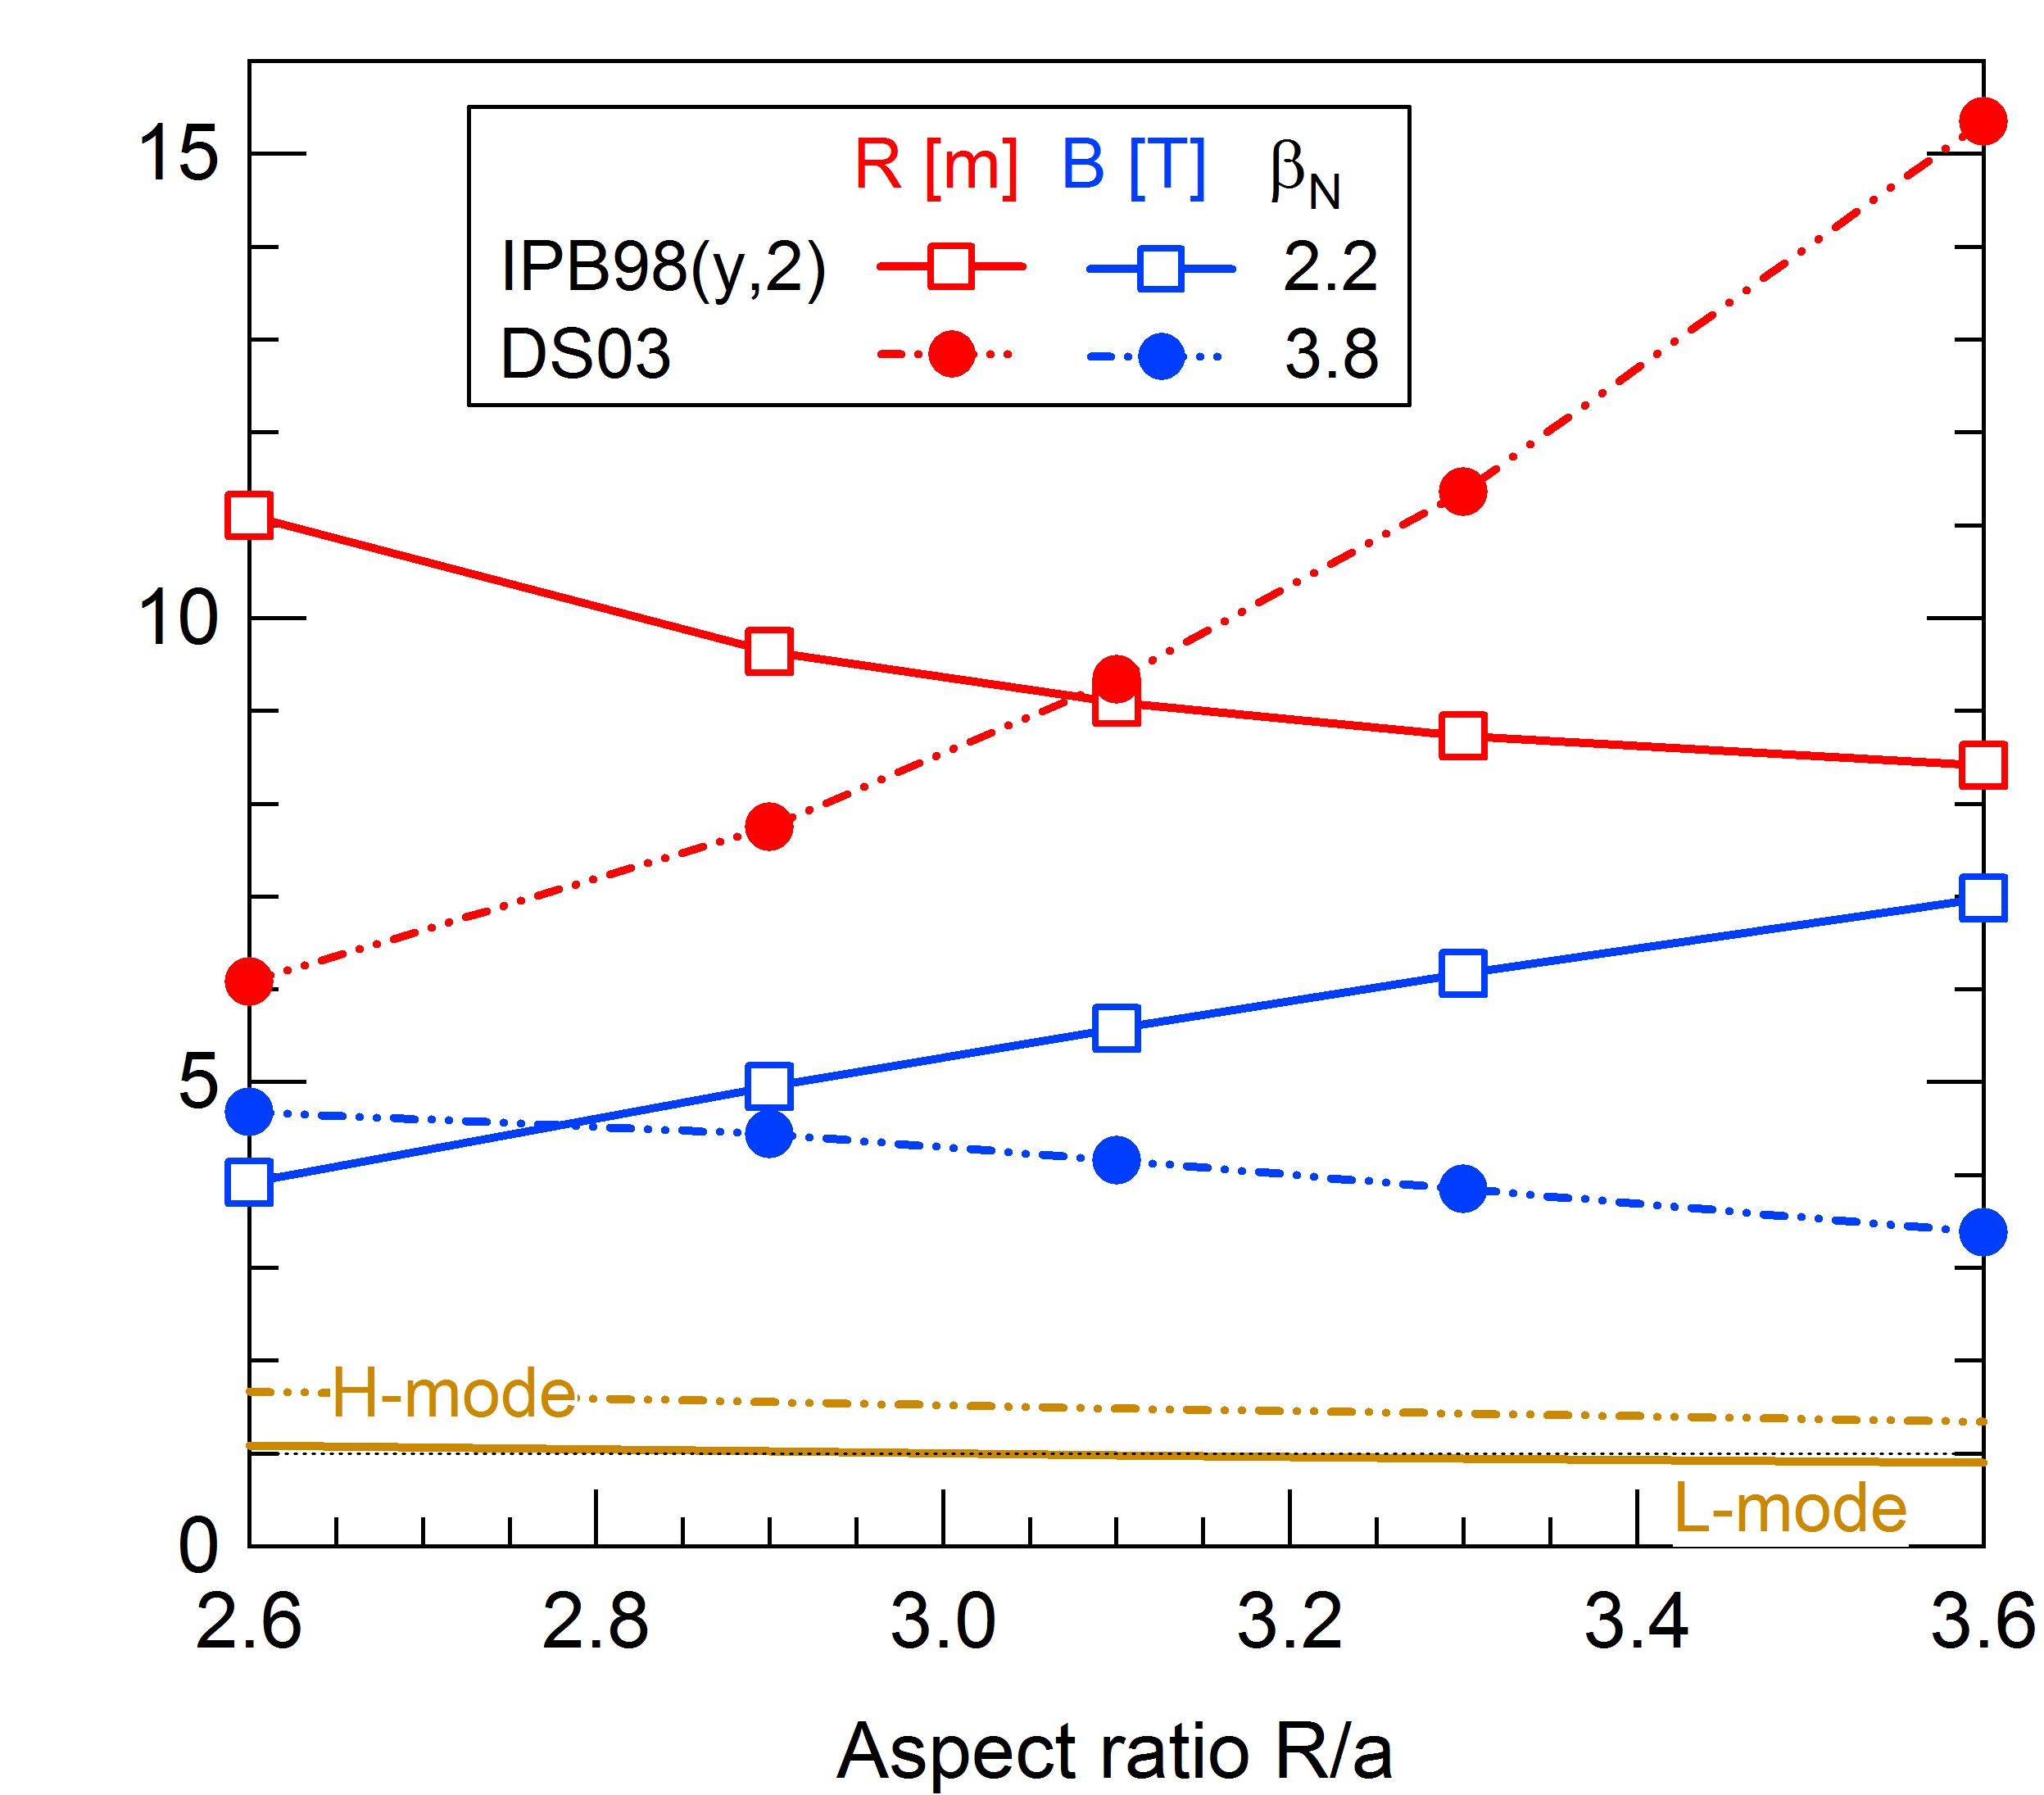
\includegraphics[width=0.55\textwidth]{DEMO_scan_A.jpg}
	\end{center}
	\caption{$R$ (red) and $B$ (blue) solutions for DEMO when varying the aspect ratio $R/a$ at fixed $\beta_N$: $\beta_N=2.2$ for the IPB98(y,2) scaling law (plain lines), and $\beta_N=3.8$ for the DS03 one (dashed lines). \newstuff{The ratio $P_{tr}/P_{L-H}$ is also plotted, in the same way as for figure \ref{fig:solutions_Hmode_DEMO}.}}
	\label{fig:solutions_scanA_DEMO}
\end{figure}

%===================================================================
\section{Conclusion} \label{sec:conclusion}
%===================================================================

A simple (mostly 0-dimensional) model is proposed for the dimensioning of tokamaks. Most of the coefficients are calculated in a comprehensive way. Given target parameters in terms of fusion gain $Q$ and fusion power $\Pfus$, and further prescribing the geometry, the model allows one to find suitable quadruplets $(R,B,n_N,\beta_N)$, i.e. the major radius, the magnetic field, the fraction of Greenwald density and the normalized $\beta$. To proceed, three scaling laws for the energy confinement time have been considered in a systematic way, valid either for L-mode (only used for DEMO design here) or for H-mode plasma regimes. When using the IPB98(y,2) scaling law, ITER typical parameters are recovered when targeting $Q=10$ and $\Pfus=500\,$MW. It is shown that some differences are obtained when using the recently published DS03 new scaling law, although the orders of magnitude are in the same range. Noticeably, the required magnetic field $B$ is smaller, while $\beta_N$ is larger. 

Also, it is shown how the uncertainty on the exponents of the $\tau_E$ scaling law, both in terms of engineering and dimensionless variables, can impact dramatically the size of the machine. Some of the most critical exponents in that respect are highlighted, pointing towards the already noticed critical role of the $\rho_*$ exponent. Finally, it is shown that a DEMO-like machine should operate at larger $\beta_N$ and lower plasma current if the DS03 scaling law holds, as compared to predictions using the IPB98(y,2) scaling. \newstuff{However, the relevance of these large $\beta_N$ plasmas for a reactor may be questioned due to their inherent larger sensitivity to MHD instabilities, and the consequent higher risk of disruptions. } Most importantly, the opposite scaling of both scaling laws with respect to the aspect ratio leads to radical differences regarding the optimal choice of this critical parameter. Especially, the DS03 law predicts that similar performance can be achieved at lower $R$ (and slightly larger $B$) when reducing $R/a$.

%===================================================================
\ack

The authors wish to acknowledge fruitful discussions with C. Reux regarding system codes in general and SYCOMORE in particular. The positive and constructive feedback received from the master students who have participated to the dimensioning project at CEA-Cadarache, France, in February 2019, is also greatly appreciated. \newstuff{Finally, we would like to acknowledge the relevant comments and useful suggestions of an anonymous referee}.

%===================================================================
\appendix

%-------------------------------------------------------------------
\section{Fusion power and momentum conservation}
\label{appendix:fusion_power}

Deuterium-tritium fusion reactions result from inelastic collisions, for which momentum is conserved, not energy. The total kinetic energy release for a single reaction amounts to $\widehat E_0 = 17.59$MeV. So as to evaluate the fraction of energy carried out by the neutron, relativistic corrections have to be taken into account. The method is detailed below.

Let's admit that it is sufficient to account for relativistic corrections for neutrons (their velocity reaches approximately $0.17\, c$, with $c$ the speed of light), while $\alpha$ particles can be treated within the classical framework (their velocity is about $0.04\, c$).
Momentum conservation then reads:
\begin{equation}
m_n \gamma_n v_n = m_\alpha v_\alpha
\label{eq:conserv_momentum}
\end{equation}
with $\gamma_n = (1-v_n^2/c^2)^{-1/2}$ the Lorentz factor for the neutrons. In the limit $\newstuff{(v_n/c)^2} \ll1$,  $\gamma_n$ can be Taylor expanded, so that (\ref{eq:conserv_momentum}) can be recast as follows: \newstuff{$u [ 1+(\epsilon/2)\, u^2 ] = 1$, } with $u \doteq v_n/(\mu v_\alpha)$, $\mu \doteq m_\alpha/m_n$ and $\epsilon \doteq \mu (v_\alpha/c)$. Since $\epsilon \ll1$, it is sufficient to look for perturbative solutions of the form: $ u = u_0 + u_1$ with $u_1\ll u_0 $. \newstuff{The approximate solution then reads: $v_n \simeq \mu v_\alpha ( 1-\epsilon^2/2)$. Injecting this expression in the kinetic energy of the neutron $E_n$ leads to: }
\begin{equation*}
	E_n = m_nc^2(\gamma_n-1) \approx 
	\frac{m_n}{2} v_n^2\left[ 1+ \frac{3v_n^2}{4c^2}\right] 
	\approx \mu\; E_\alpha \left( 1-\frac{\epsilon^2}{4}\right)
\end{equation*}
The kinetic energy of the $\alpha$ particle $E_\alpha$ can then be expressed as a function of the total energy $E_0$ ($E_0 =E_\alpha + E_n$):
\begin{equation}
E_\alpha^2 - \frac{2(1+\mu)}{\mu^2}E_{n0}\, E_\alpha + \frac{2}{\mu^2}\; E_{n0}E_0 = 0
\end{equation}
\newstuff{with $E_{n0} = m_nc^2$ } the mass energy of the neutron \newstuff{and using } the relation $\epsilon^2 = 2\mu\; E_\alpha/E_{n0}$. The only acceptable solution is:
\begin{equation}
E_\alpha = \frac{1+\mu}{\mu^2}
\left( 1 - \sqrt{1-\frac{2\mu^2}{(1+\mu)^2}\frac{E_0}{E_{n0}}}\right)\; E_{n0}
\end{equation}
\newstuff{At } leading order in $E_0/E_{n0}\ll1$, this solution simply reduces to $E_\alpha \approx E_0/(1+\mu) \approx E_0/5$. \newstuff{Notice } that $\mu\neq 4$. 
Indeed, the mass of the $\alpha$ particle is slightly less than the sum of its components (actually, this mass difference $\Delta m \approx 0.0187\; m_p$ is the one which leads to the energy release of the D-T fusion reaction $E_0 = \Delta m\;c^2$). The masses can be found in reference \cite{Wesson2004}. In particular, $m_n \approx (1+0.001378)\, m_p$ and \newstuff{$\mu \doteq m_\alpha/m_n \approx (1-0.027404)\; m_p /m_n \approx 3.967$. }
With these data, one finally obtains $E_0/E_\alpha \approx 4.94$ and $\widehat E_\alpha \approx 3.56\,$MeV.


%-------------------------------------------------------------------
\section{Fraction of $\alpha$ particles}
\label{appendix:alpha_particles}

The total number $N_\alpha = n_\alpha V_t$ of $\alpha$ particles in the confined plasma can be estimated from the following balance equation: 
\begin{equation}
\frac{N_\alpha}{\tau_\alpha} = S_\alpha + R_\alpha\; \frac{N_\alpha}{\tau_\alpha}
\end{equation}
The left hand side accounts for the radial transport due to both turbulence and collisions, with the characteristic time $\tau_\alpha$. The right hand side represents the sources: the volumetric source due to D-T fusion reactions, and the wall recycling characterized by the coefficient $0 \leq R_\alpha \leq 1$. $R_\alpha$ accounts for the pumping efficiency of the $\alpha$ particle pumps installed in the divertor. The effective confinement time of the $\alpha$ particles then reads $\tau_\alpha^* = \tau_\alpha / (1-R_\alpha)$.

$S_\alpha$ reads as follows (for $T$ in the range 10.3-18.5 keV):
\begin{equation}
S_\alpha = n_D N_T \langle \sigma v\rangle V_t \approx \frac{1.18\, 10^{14}}{4}\; (\widehat n \widehat T)^2  V_t
\end{equation}
Without any obvious estimate for $\tau_\alpha^*$, it is usually assumed to scale with $\tau_E$: $\tau_\alpha^* \sim C_\alpha \tau_E$, with typical values in the range $C_\alpha < 5-10$ in H-mode \cite[section 2.3]{ITERphysics_chap4} (particle confinement times are usually larger than the one of energy because the later has several transport channels (convection and conduction) whereas particle transport is due to convection only).

The fraction of $\alpha$ particles then simply reads:
\begin{equation}
f_\alpha \doteq \frac{n_\alpha}{n} \approx \frac{1.18\, 10^{-5}C_\alpha}{4}\; \widehat n \widehat T^2 \tau_E
\end{equation}
Taking ITER parameters given in section~\ref{subsec:ITER_characteristics} and $C_\alpha=4.65$, one finds $f_\alpha \approx 3.5\%$, which is the fraction we have considered for ITER. The fraction considered for DEMO $f_\alpha =10\%$ is also consistent with the values obtained for density, temperature and confinement time, with $C_\alpha \approx 4$.

%===================================================================
\vspace{10pt}
\bibliographystyle{unsrt}
\bibliography{references}
%===================================================================
\end{document}

